\documentclass[11pt]{article}

\usepackage[margin=1in]{geometry}
\usepackage[T1]{fontenc}
\usepackage{lmodern}
\usepackage{microtype}
\usepackage{amsmath, amssymb}
\usepackage{graphicx}
\usepackage{booktabs}
\usepackage{longtable}
\usepackage{array}
\usepackage{enumitem}
\usepackage{xcolor}
\usepackage{hyperref}
\usepackage{caption}
\usepackage{subcaption}
\usepackage{float}
\usepackage{listings}
\usepackage{tikz}
\usepackage[most]{tcolorbox}
\usepackage{setspace}
\usetikzlibrary{arrows.meta,positioning,calc}

\hypersetup{
  colorlinks=true,
  linkcolor=blue!55!black,
  urlcolor=blue!55!black,
  citecolor=blue!55!black
}

\definecolor{codebg}{RGB}{248,250,252}
\definecolor{codeframe}{RGB}{203,213,225}
\definecolor{concept}{RGB}{30,64,175}
\definecolor{warning}{RGB}{146,64,14}
\definecolor{good}{RGB}{22,101,52}

\newcommand{\code}[1]{\texttt{\detokenize{#1}}}
\newcommand{\vect}[1]{\boldsymbol{#1}}
\newcommand{\R}{\mathbb{R}}
\setstretch{1.1}
\setlength{\parskip}{0.25\baselineskip}

\lstdefinestyle{pythonstyle}{
  language=Python,
  basicstyle=\ttfamily\footnotesize,
  backgroundcolor=\color{codebg},
  frame=single,
  rulecolor=\color{codeframe},
  breaklines=true,
  showstringspaces=false,
  tabsize=4,
  columns=fullflexible
}
\lstset{style=pythonstyle}

\newtcolorbox{conceptbox}[1]{
  enhanced,
  colback=blue!3,
  colframe=concept!75!black,
  title=#1,
  fonttitle=\bfseries,
  boxrule=0.7pt,
  arc=2pt
}

\newtcolorbox{warningbox}[1]{
  enhanced,
  colback=orange!5,
  colframe=warning,
  title=#1,
  fonttitle=\bfseries,
  boxrule=0.7pt,
  arc=2pt
}

\newtcolorbox{labbox}[1]{
  enhanced,
  colback=green!4,
  colframe=good,
  title=#1,
  fonttitle=\bfseries,
  boxrule=0.7pt,
  arc=2pt
}

\title{\textbf{Training and Evaluating the Rowing Force-Curve Model}\\
\large A Math-Focused Study Guide for the \code{rowing-video-analysis} Pipeline}
\author{Repository study guide}
\date{\today}

\begin{document}
\maketitle
\tableofcontents
\newpage

\section*{How to Use This Guide}
\addcontentsline{toc}{section}{How to Use This Guide}

This guide explains the part of the repository that turns prepared rowing
training data into force-curve predictors and evaluates whether those predictors
are actually useful. It assumes you know basic probability, statistics, and
Python, but it does not assume that you are already comfortable reading a
multi-stage machine-learning pipeline.

The most important source files are:
\begin{itemize}[leftmargin=*]
  \item \code{src/rowing/dataset/build.py}: builds the supervised training dataset.
  \item \code{src/rowing/modeling/train.py}: trains Stage 0, Stage A, and Stage B models.
  \item \code{src/rowing/modeling/eval_metrics.py}: computes splits, metrics, and evaluation-regime warnings.
  \item \code{src/rowing/dataset/segment_features.py}: shows how video-derived pose features become model input sequences.
\end{itemize}

The upstream pose extraction, RP3 matching, and segment export system matters
because it defines the meaning of the data. However, this guide focuses on the
training and evaluation path. Whenever we refer to a ``stroke,'' we mean a
single drive phase that has already been aligned to a corresponding RP3 force
curve.

\begin{conceptbox}{Central Mental Model}
Every supervised sample is one stroke. The model sees a progress-indexed
description of the rower's motion, \(X_i(s)\), and tries to predict the
corresponding force curve, \(Y_i(s)\), over the drive. The hard part is not just
fitting a model; it is proving that the model learned useful biomechanics rather
than memorizing session-specific artifacts.
\end{conceptbox}

\subsection*{Code-to-Math Map}
\addcontentsline{toc}{subsection}{Code-to-Math Map}

The table below is the fastest way to connect the repository's objects to the
mathematical notation used later in the guide.

\begin{longtable}{p{0.28\linewidth}p{0.20\linewidth}p{0.42\linewidth}}
\toprule
\textbf{Repository object} & \textbf{Notation} & \textbf{Study meaning}\\
\midrule
\endhead
\code{kinematic_sequences[i]} & \(X_i\) & One stroke's full progress-aligned
input tensor, shaped \(G \times K\).\\
\code{force_curves[i]} & \(Y_i\) & One stroke's target force curve on the same
\(s\)-grid.\\
\code{s_grid} & \((s_1,\ldots,s_G)\) & Shared progress coordinate from catch
to finish.\\
\code{strokes_df.iloc[i]} & metadata row & Scalar context for a stroke:
rate, length, drive time, QC status, run, athlete.\\
\code{pca_0}, \code{pca_1}, \(\ldots\) & \(c_{i1},c_{i2},\ldots\) & Low-dimensional
force-shape coordinates used by Stage 0 and Stage A.\\
\code{cv_predictions/*.npy} & \(\hat{Y}^{\text{CV}}\) & Held-out predictions
assembled fold by fold; these are the predictions used for honest metrics.\\
\bottomrule
\end{longtable}

When reading the code, keep one invariant in mind: row \(i\) in
\code{strokes.csv}, row \(i\) in \code{force_curves_resampled.npy}, and slice
\(i\) in \code{kinematic_sequences.npy} all describe the same stroke after the
dataset has been assembled. If this alignment is broken, even a perfectly
implemented model will train on the wrong labels.

\clearpage
\section{ML Problem Setup}

\subsection{From Rowing Stroke to Supervised Sample}

In a standard introductory statistics course, an observation might be a scalar
random variable \(X\), and the goal might be to estimate a mean or predict a
scalar label \(Y\). In this project, one observation is richer: one rowing
stroke produces an entire sequence of kinematic measurements and an entire
force curve.

For stroke \(i\), define:
\[
  X_i(s) \in \R^K, \qquad Y_i(s) \in \R,
  \qquad s \in [0,1].
\]
Here \(s\) is normalized drive progress: \(s=0\) means catch, and \(s=1\)
means finish. The input \(X_i(s)\) contains \(K\) channels such as active-side
knee angle, hip angle, elbow angle, trunk angle, progress derivatives, and
handle velocity. The target \(Y_i(s)\) is the RP3 force at that same fraction
of the drive.

In code, the continuous functions are represented on a grid:
\[
  s_1, s_2, \ldots, s_G,
  \qquad G=64 \text{ by default}.
\]
Thus one input sample becomes a matrix:
\[
  X_i =
  \begin{bmatrix}
  x_{i,1,1} & x_{i,1,2} & \cdots & x_{i,1,K}\\
  x_{i,2,1} & x_{i,2,2} & \cdots & x_{i,2,K}\\
  \vdots & \vdots & \ddots & \vdots\\
  x_{i,G,1} & x_{i,G,2} & \cdots & x_{i,G,K}
  \end{bmatrix}
  \in \R^{G \times K}.
\]
The full training set is stored as a 3D tensor:
\[
  X \in \R^{N \times G \times K},
\]
where \(N\) is the number of strokes after quality control. The target force
curves are stored as:
\[
  Y \in \R^{N \times G}.
\]

\begin{figure}[H]
  \centering
  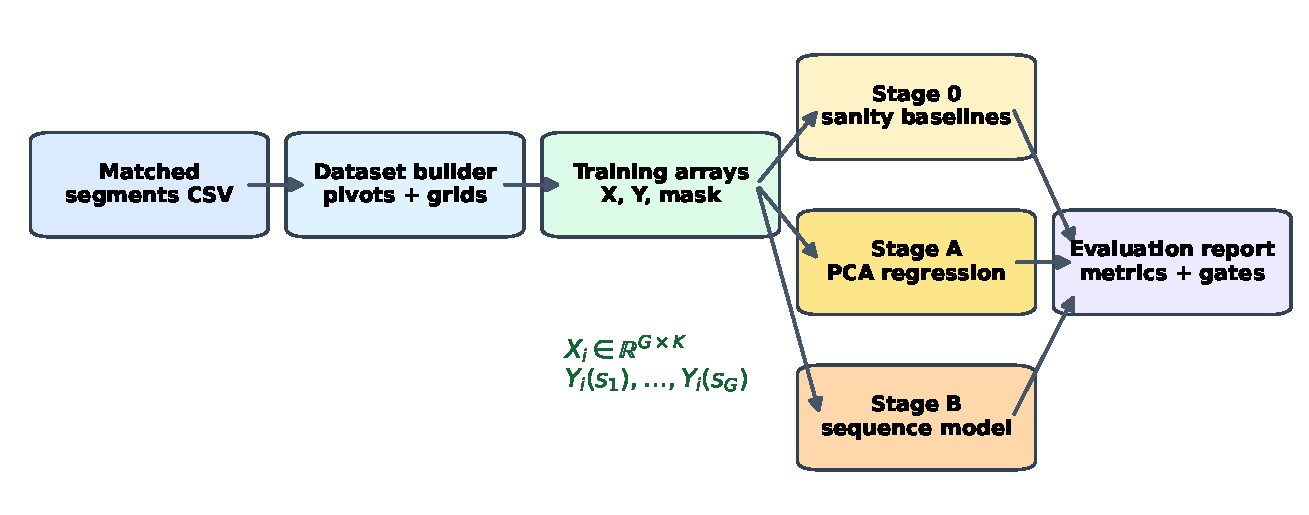
\includegraphics[width=0.98\linewidth]{figures/training_flow.pdf}
  \caption{High-level training flow from matched segments to model evaluation.}
  \label{fig:training-flow}
\end{figure}

\subsection{What Is Being Learned?}

The ideal predictor is a function \(f^\star\) that maps a stroke's motion to a
force curve:
\[
  f^\star: \R^{G \times K} \rightarrow \R^G.
\]
Given training data
\[
  \mathcal{D}=\{(X_i,Y_i)\}_{i=1}^{N},
\]
the pipeline learns an approximation \(\hat{f}\). A fitted model is successful
only if \(\hat{f}(X)\) works on held-out strokes that were not used to fit the
model.

This is supervised regression. It is not classification because the label is
not a discrete class such as ``good'' or ``bad.'' It is not scalar regression
because the label is not just one number. It is vector-valued regression:
\[
  \hat{Y}_i =
  \begin{bmatrix}
  \hat{Y}_i(s_1) & \cdots & \hat{Y}_i(s_G)
  \end{bmatrix}.
\]

\subsection{A Tiny Numerical Example}

Suppose we used only four grid points instead of 64:
\[
  s = [0,\;0.33,\;0.67,\;1.0].
\]
For one stroke, a simplified input might contain knee and hip angles:
\[
  X_i =
  \begin{bmatrix}
    58 & 42\\
    92 & 55\\
    128 & 69\\
    151 & 79
  \end{bmatrix}.
\]
The target might be a force curve:
\[
  Y_i =
  \begin{bmatrix}
    0 & 410 & 520 & 70
  \end{bmatrix}.
\]
In the real dataset, \(G=64\), \(K\) is typically around 14, and the target has
64 force values. But the learning question is the same: given the whole matrix
\(X_i\), predict the whole vector \(Y_i\).

This example also explains why a normal spreadsheet view is not enough. A
single row in \code{strokes.csv} cannot hold all information in \(X_i\) unless
the sequence has been summarized. Stage A deliberately uses summaries. Stage B
uses the full matrix.

\begin{conceptbox}{Regression Is Estimation}
In probability language, the ideal squared-error predictor is the conditional
expectation \(f^\star(X)=\mathbb{E}[Y\mid X]\). The repository does not know
the true conditional distribution, so it estimates a useful approximation from
paired examples.
\end{conceptbox}

\subsection{Training vs Inference}

During training, two streams are synchronized:
\begin{itemize}[leftmargin=*]
  \item video-derived kinematics, which become \(X_i(s)\);
  \item RP3 force curves, which become \(Y_i(s)\).
\end{itemize}
During video-only inference, RP3 data is absent. The trained model uses the
same feature contract to build \(X_i(s)\) from video and predicts
\(\hat{Y}_i(s)\). This separation is scientifically important: RP3 is the
teacher during training, not an input at deployment.

\begin{warningbox}{Do Not Confuse Supervision With Inference Input}
The model is allowed to see RP3 force curves while learning because those force
curves provide labels. A deployed predictor must not require RP3 force curves as
features. If the label leaks into the input, evaluation becomes meaningless.
\end{warningbox}

\subsection{Why Normalized Drive Progress?}

A rowing drive has two natural axes: time and distance/progress. Two strokes
may have different drive durations but similar mechanical phases. If one stroke
takes \(0.75\) seconds and another takes \(0.95\) seconds, comparing them at the
same wall-clock time does not necessarily compare the same part of the drive.

The repository therefore uses normalized drive progress:
\[
  s = \frac{\text{progress since catch}}{\text{progress at finish} -
  \text{progress at catch}}.
\]
This makes the learning problem closer to: ``given body configuration at this
part of the drive, predict force at this part of the drive.''

\clearpage
\section{Dataset Contract}

\subsection{The Training Dataset Directory}

The dataset builder consumes one or more long-form segment CSV files. Each
row in those segment CSVs corresponds to one force bin within one matched
stroke. The builder pivots those rows into stroke-level arrays and writes a
training dataset directory.

The key function is \code{build_training_dataset} in
\code{src/rowing/dataset/build.py}. Its output is a contract between feature
engineering and modeling. If you understand this directory, you can understand
the rest of the training code.

\begin{longtable}{p{0.32\linewidth}p{0.18\linewidth}p{0.42\linewidth}}
\toprule
\textbf{Artifact} & \textbf{Shape} & \textbf{Meaning}\\
\midrule
\endhead
\code{strokes.csv} & \(N\) rows & One row per stroke: metadata, QC flags,
PCA/fPCA coefficients, scalar kinematic features, and coordination features.\\
\code{force_curves_resampled.npy} & \(N \times G\) & Raw force in Newtons on
the fixed \(s\)-grid. This is the main direct curve target.\\
\code{force_curves_peak_norm.npy} & \(N \times G\) & Force curves divided by
their own peak. Used to fit PCA shape targets.\\
\code{force_curves_padded.npy} & \(N \times 77\) & Native RP3 2.2 cm bins,
padded with NaN beyond actual stroke length.\\
\code{force_mask.npy} & \(N \times 77\) & Boolean mask marking valid native
bins.\\
\code{kinematic_sequences.npy} & \(N \times G \times K\) & Fixed-grid input
sequence tensor.\\
\code{kinematic_padded.npy} & \(N \times 77 \times K\) & Native-bin kinematic
features aligned to RP3 bins.\\
\code{s_grid.npy} & \(G\) & The common progress grid from 0 to 1.\\
\code{pca_model.joblib} & object & Fitted scikit-learn PCA model for
peak-normalized force curves.\\
\code{feature_names.json} & list & Ordered names for the channels in
\code{kinematic_sequences.npy}.\\
\code{dataset_summary.json} & object & Provenance, QC counts, grid sizes,
and included runs/athletes.\\
\bottomrule
\end{longtable}

\subsection{DataFrames, Arrays, and Serialized Models}

The repository uses three main data representations.

\textbf{Pandas DataFrames} are tabular. They are good for metadata: stroke
rate, athlete ID, run name, QC flags, and one scalar per row. The main example
is \code{strokes.csv}.

\textbf{NumPy arrays} are dense numerical tensors. They are good for model
inputs and targets because shape matters. The main examples are
\code{force_curves_resampled.npy} and \code{kinematic_sequences.npy}.

\textbf{Serialized model objects} store learned transformations. The main
example is \code{pca_model.joblib}, which saves the PCA mean vector,
component matrix, and other state needed to transform and reconstruct curves.

\subsection{What the Modeling Script Loads}

The training script does not rebuild features. It trusts the dataset directory
and loads a fixed set of artifacts:

\begin{lstlisting}
d["strokes_df"] = pd.read_csv(dataset_dir / "strokes.csv")
d["force_curves"] = np.load(dataset_dir / "force_curves_resampled.npy")
d["force_peak_norm"] = np.load(dataset_dir / "force_curves_peak_norm.npy")
d["kinematic_sequences"] = np.load(dataset_dir / "kinematic_sequences.npy")
d["s_grid"] = np.load(dataset_dir / "s_grid.npy")
d["pca_model"] = joblib.load(dataset_dir / "pca_model.joblib")
\end{lstlisting}

This division of labor is useful. Feature engineering is expensive and
domain-specific, while model training is an experiment that may be rerun many
times with different stages, split methods, or hyperparameters. By saving a
dataset contract, the project can train models without redoing pose processing
or RP3 matching.

The separation also creates a responsibility: if you change feature extraction,
QC thresholds, grid size, or target representation, you must rebuild the dataset
before comparing model results. Otherwise, two modeling runs may not be
answering the same question.

\begin{conceptbox}{Shape Check}
The most useful first debugging question is: ``What is the shape?'' If
\code{kinematic_sequences.shape == (N, G, K)} and
\code{force_curves_resampled.shape == (N, G)}, then the \(i\)th input sequence
and the \(i\)th target curve refer to the same stroke.
\end{conceptbox}

\subsection{How Long-Form Rows Become Stroke-Level Samples}

The builder starts by loading segment CSVs and grouping by run and matched
stroke index:

\begin{lstlisting}
group_cols = ["run_name", "match_seq_idx"]
for (run_name, seq_idx), grp in df.groupby(group_cols, sort=False):
    grp = grp.sort_values("s_force").reset_index(drop=True)
    record["s_force_arr"] = grp["s_force"].to_numpy(dtype=np.float64)
    record["force_raw_arr"] = grp["force_raw"].to_numpy(dtype=np.float64)
\end{lstlisting}

Conceptually, a long table like this:
\[
  \text{stroke},\quad s,\quad F(s),\quad \theta_{\text{knee}}(s),\ldots
\]
is turned into one Python record per stroke. That record contains arrays:
\[
  \bigl[s_1,\ldots,s_m\bigr],
  \qquad
  \bigl[F(s_1),\ldots,F(s_m)\bigr],
  \qquad
  \bigl[\theta(s_1),\ldots,\theta(s_m)\bigr].
\]

\subsection{Quality Control}

Machine learning code can fit almost anything, including bad labels and noisy
features. The dataset builder therefore marks or drops questionable strokes.
Important flags include:
\begin{itemize}[leftmargin=*]
  \item \code{qc_tracking_sparse}: too many missing pose/angle values.
  \item \code{qc_nonphysio_deriv}: implausibly large angular velocity.
  \item \code{qc_duration_implausible}: drive or cycle duration outside
  expected range.
  \item \code{qc_alignment_drift}: video/RP3 cumulative catch timing drift is
  too large.
  \item \code{qc_rate_mismatch}: video and RP3 stroke rates disagree too much.
\end{itemize}

The builder supports soft and hard QC. In soft mode, flagged strokes are kept
but marked. In hard mode, flagged strokes are removed before the arrays are
written. The training script also filters \code{qc_excluded} rows when deciding
which strokes are valid.

\subsection{Study Check: Reading a Dataset Summary}

When you open \code{dataset_summary.json}, look for these fields first:
\begin{itemize}[leftmargin=*]
  \item \code{n_strokes_before_qc} and \code{n_strokes_after_qc}: how much data
  survived filtering?
  \item \code{qc_mode}: were flagged strokes retained or removed?
  \item \code{n_grid}: does it match the model bundle and notebooks?
  \item \code{n_pca_components}: how many shape coefficients were created?
  \item \code{pca_total_explained_variance}: how much normalized force-shape
  variability is retained?
  \item \code{runs_included} and \code{athletes_included}: what generalization
  claim is even possible?
\end{itemize}

If the dataset contains one athlete, athlete-held-out evaluation is impossible.
If it contains one session, session-held-out evaluation is impossible. The
right split strategy is constrained by the data that actually exists.

\clearpage
\section{Feature and Target Representation}

\subsection{Feature Families}

The fixed-grid feature tensor contains angle channels, progress-derivative
channels, and handle support channels. The default feature names in
\code{build.py} are:
\[
\begin{split}
&\code{knee_active_deg},\code{hip_active_deg},\code{elbow_active_deg},\\
&\code{trunk_vs_horizontal_deg},\code{spine_flexion_deg},
\code{head_vs_trunk_deg},
\end{split}
\]
then first derivatives such as \code{knee_active_ddeg_ds}, plus
\code{handle_velocity_px_s} and \code{handle_accel_px_s2}.

The active-side names are deliberate. Instead of asking the model to separately
learn left-knee and right-knee conventions, each session declares an
\code{active_side}, and the feature contract maps source columns to canonical
names. This makes the data more comparable across camera views.

\subsection{Mirror Normalization}

Most joint angles are flexion magnitudes in degrees. They are symmetric under
left/right image flips. The trunk orientation, however, is measured relative to
the image horizontal axis. If the rower faces the opposite direction, the same
physical posture can produce a supplementary angle. The mirror policy applies:
\[
  \theta_{\text{trunk, canonical}} =
  \begin{cases}
    180^\circ - \theta_{\text{trunk}}, & \text{if rower faces left},\\
    \theta_{\text{trunk}}, & \text{otherwise}.
  \end{cases}
\]

The source file \code{feature_contract.py} centralizes this policy so training
and inference use the same convention.

\begin{lstlisting}
def mirror_transform(canonical_name, values, *, facing):
    arr = np.asarray(values, dtype=np.float64).copy()
    if facing != "left":
        return arr
    if policy.kind == "supplement_180":
        return 180.0 - arr
    return arr
\end{lstlisting}

\subsection{Interpolation Onto a Common Grid}

Video frames do not naturally occur at the same \(s\)-values as RP3 force bins.
The pipeline therefore interpolates video-derived features onto target progress
locations. The central operation is linear interpolation:
\[
  \hat{x}(s^\star) =
  x(s_a) +
  \frac{s^\star-s_a}{s_b-s_a}
  \bigl(x(s_b)-x(s_a)\bigr),
\]
where \(s_a \le s^\star \le s_b\). In code, this is handled by
\code{np.interp} after sorting, clipping, and enforcing monotonic progress.

\begin{lstlisting}
valid = np.isfinite(arr_s) & np.isfinite(arr_v)
return np.interp(s_grid, arr_s[valid], arr_v[valid])
\end{lstlisting}

This step is not just a convenience. It defines the model's coordinate system.
Every stroke becomes comparable because every stroke is represented at the same
progress values \(s_1,\ldots,s_G\).

\subsection{Smoothing and Derivatives}

Pose-derived angles can be noisy. Derivatives amplify noise, so the pipeline
uses light Savitzky-Golay smoothing before differentiating. For an angle
\(\theta(t)\), the code first estimates \(d\theta/dt\). It also estimates
\(ds/dt\), the rate of progress through the drive. The progress-domain
derivative is computed by the chain rule:
\[
  \frac{d\theta}{ds}
  =
  \frac{d\theta/dt}{ds/dt + \epsilon}.
\]
The small \(\epsilon\) prevents division by zero when progress nearly stalls.
The code also flags strokes when \(ds/dt\) is unstable or when derivatives are
non-physiologically large.

\begin{lstlisting}
ds_dt_on_s = _interp_on_progress(s_video, ds_dt_time, s_grid)
dtheta_dt_on_s = _interp_on_progress(s_video, dtheta_dt[name], s_grid)
dtheta_ds = dtheta_dt_on_s / (ds_dt_on_s + CHAIN_RULE_EPS)
\end{lstlisting}

\begin{figure}[H]
  \centering
  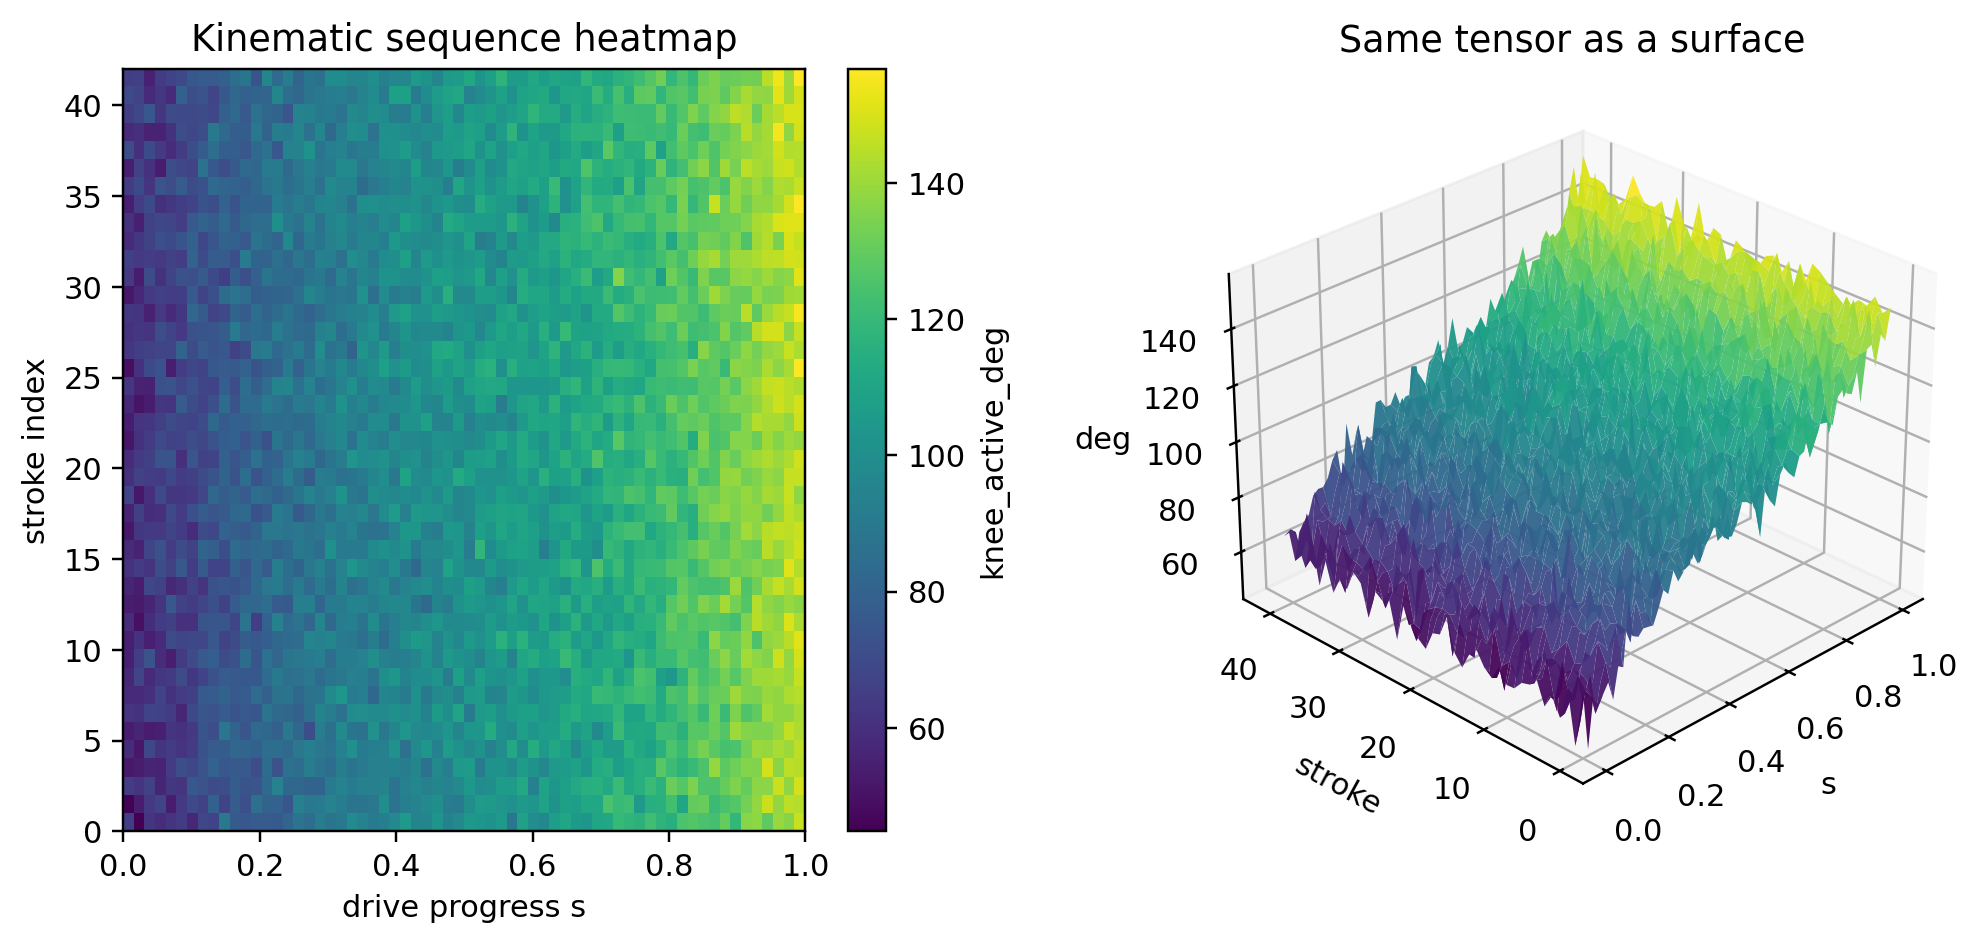
\includegraphics[width=0.95\linewidth]{figures/feature_heatmap.png}
  \caption{The sequence tensor can be viewed as a heatmap or as a 3D surface.}
  \label{fig:feature-heatmap}
\end{figure}

\subsection{Target Representation 1: Native Padded Bins}

RP3 force curves are sampled every 2.2 cm up to a maximum distance. Not every
stroke reaches the maximum length, so the native representation is padded:
\[
  Y_{\text{native}} \in \R^{N \times 77}.
\]
Invalid bins are NaN, and a boolean mask marks valid bins. This representation
preserves the native RP3 sampling. It is especially relevant for masked losses:
\[
  L_{\text{masked}}
  =
  \frac{\sum_{i,g} m_{ig}(\hat{y}_{ig}-y_{ig})^2}
  {\sum_{i,g} m_{ig}},
\]
where \(m_{ig}=1\) if bin \(g\) is valid for stroke \(i\).

\subsection{Target Representation 2: Fixed-Grid Curves}

The sequence models and PCA code use fixed-grid curves:
\[
  Y_{\text{grid}} \in \R^{N \times G}.
\]
The default is \(G=64\), which is close to the native number of RP3 bins for a
typical drive. This makes the force target match the kinematic sequence grid.

The builder applies the same operation to force and every kinematic feature:

\begin{lstlisting}
force_resampled[i] = _resample_to_grid(s_arr, f_arr, s_grid)
for k, feat_col in enumerate(KINEMATIC_FEATURE_COLS):
    kinematic_sequences[i, :, k] = _resample_to_grid(
        s_arr, s[f"{feat_col}_arr"], s_grid
    )
\end{lstlisting}

This is one of the most important invariants in the repository: the target and
the features are not just the same length; they are indexed by the same physical
meaning. Column \(g\) in the target curve is force at \(s_g\). Row \(g\) in the
kinematic sequence is body motion at \(s_g\).

\begin{figure}[H]
  \centering
  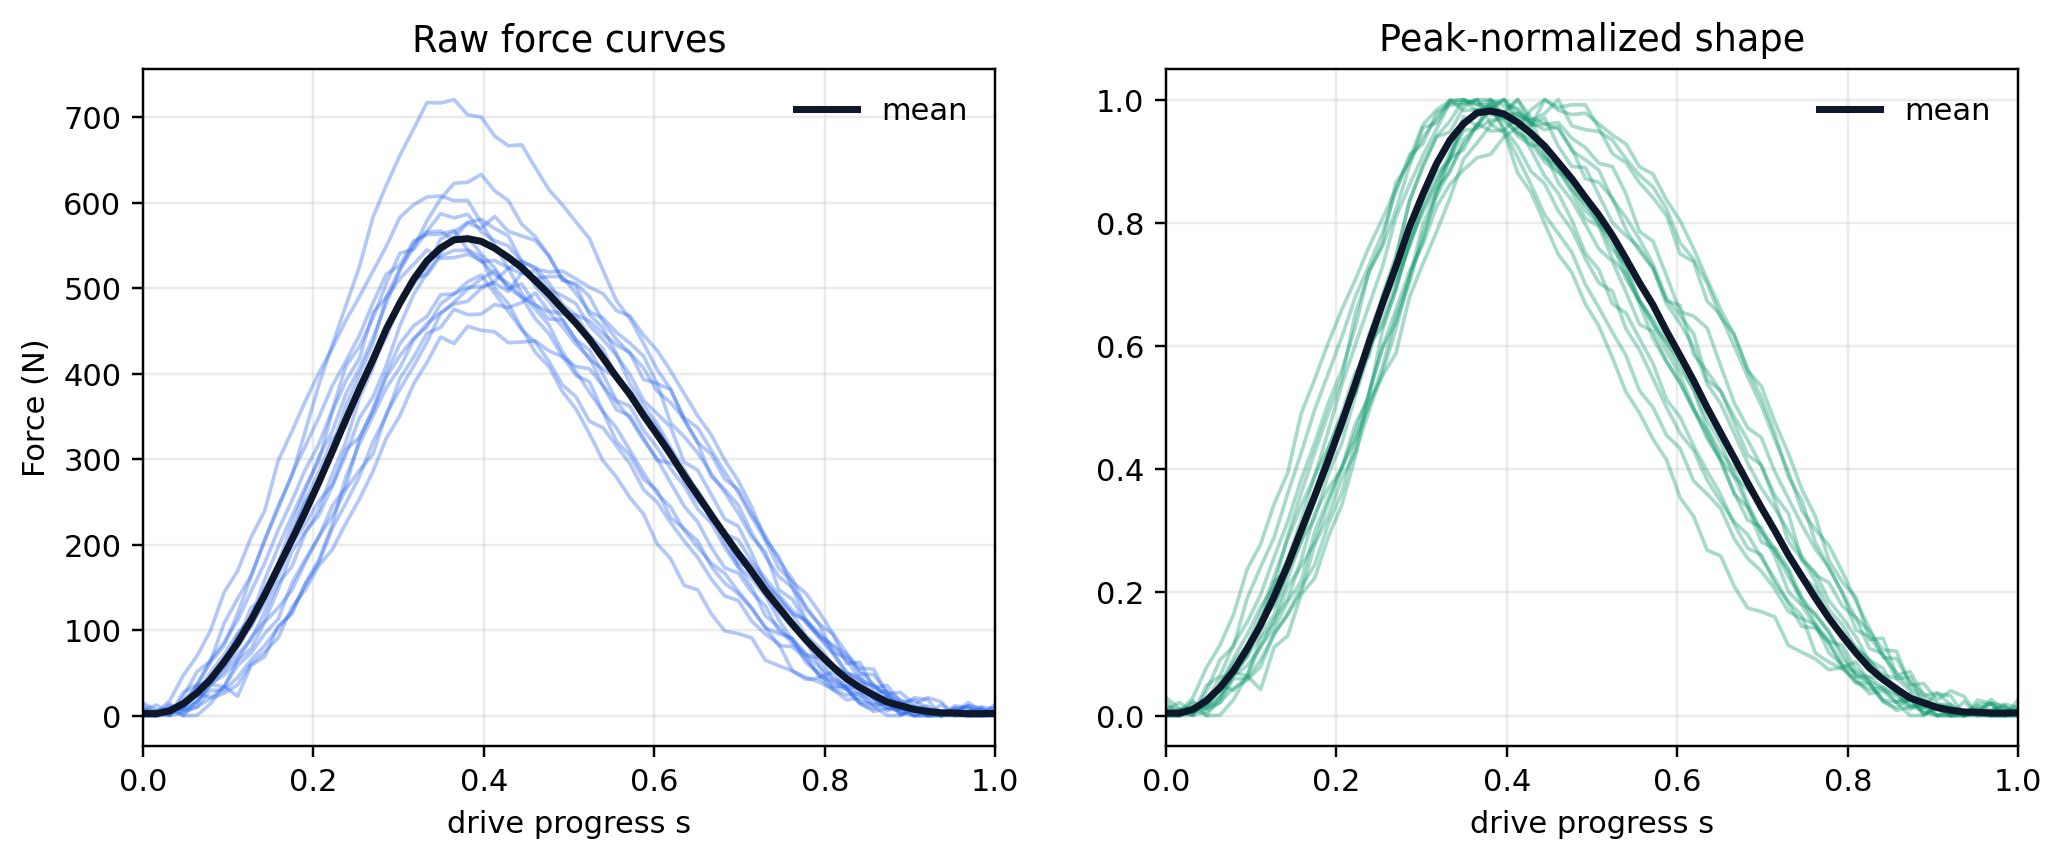
\includegraphics[width=0.95\linewidth]{figures/force_curves.png}
  \caption{Raw force curves preserve absolute scale; peak-normalized curves
  emphasize shape.}
  \label{fig:force-curves}
\end{figure}

\subsection{Peak Normalization}

PCA is fitted to peak-normalized curves:
\[
  \tilde{Y}_i(s_g)
  =
  \frac{Y_i(s_g)}{\max_h Y_i(s_h)}.
\]
This makes PCA primarily describe shape rather than absolute magnitude. The
metadata and kinematic models then predict PCA coefficients for the normalized
shape. During evaluation, reconstruction can be rescaled by peak force when
available.

\subsection{PCA as a Low-Dimensional Shape Model}

Principal component analysis finds directions of maximum variance in a dataset.
Let \(\tilde{\vect{y}}_i \in \R^G\) be the peak-normalized force curve for
stroke \(i\). PCA writes an approximate curve as:
\[
  \tilde{\vect{y}}_i
  \approx
  \vect{\mu}
  +
  c_{i1}\vect{v}_1
  +
  \cdots
  +
  c_{iq}\vect{v}_q,
\]
where \(\vect{\mu}\) is the mean curve, \(\vect{v}_j\) are principal component
directions, and \(c_{ij}\) are scores. Stage 0 and Stage A models predict the
scores \(c_{ij}\), not every force grid point directly.

\begin{lstlisting}
pca = PCA(n_components=n_components, whiten=False)
pca.fit(force_peak_norm[valid_max])
pca_coeffs[valid_max] = pca.transform(force_peak_norm[valid_max])
\end{lstlisting}

PCA is compression, not prediction. It only builds a coordinate system for
already-observed force curves. The learning model still has to predict where a
new stroke lies in that coordinate system.

For example, if \(q=5\), Stage A predicts:
\[
  \hat{\vect{c}}_i =
  [\hat{c}_{i1},\hat{c}_{i2},\hat{c}_{i3},\hat{c}_{i4},\hat{c}_{i5}].
\]
The PCA inverse transform then converts those five numbers back into a
64-point curve. If the first few components explain most force-shape variance,
this is efficient. If important shape details live in discarded components,
Stage A cannot recover them no matter how good the regressor is.

\begin{figure}[H]
  \centering
  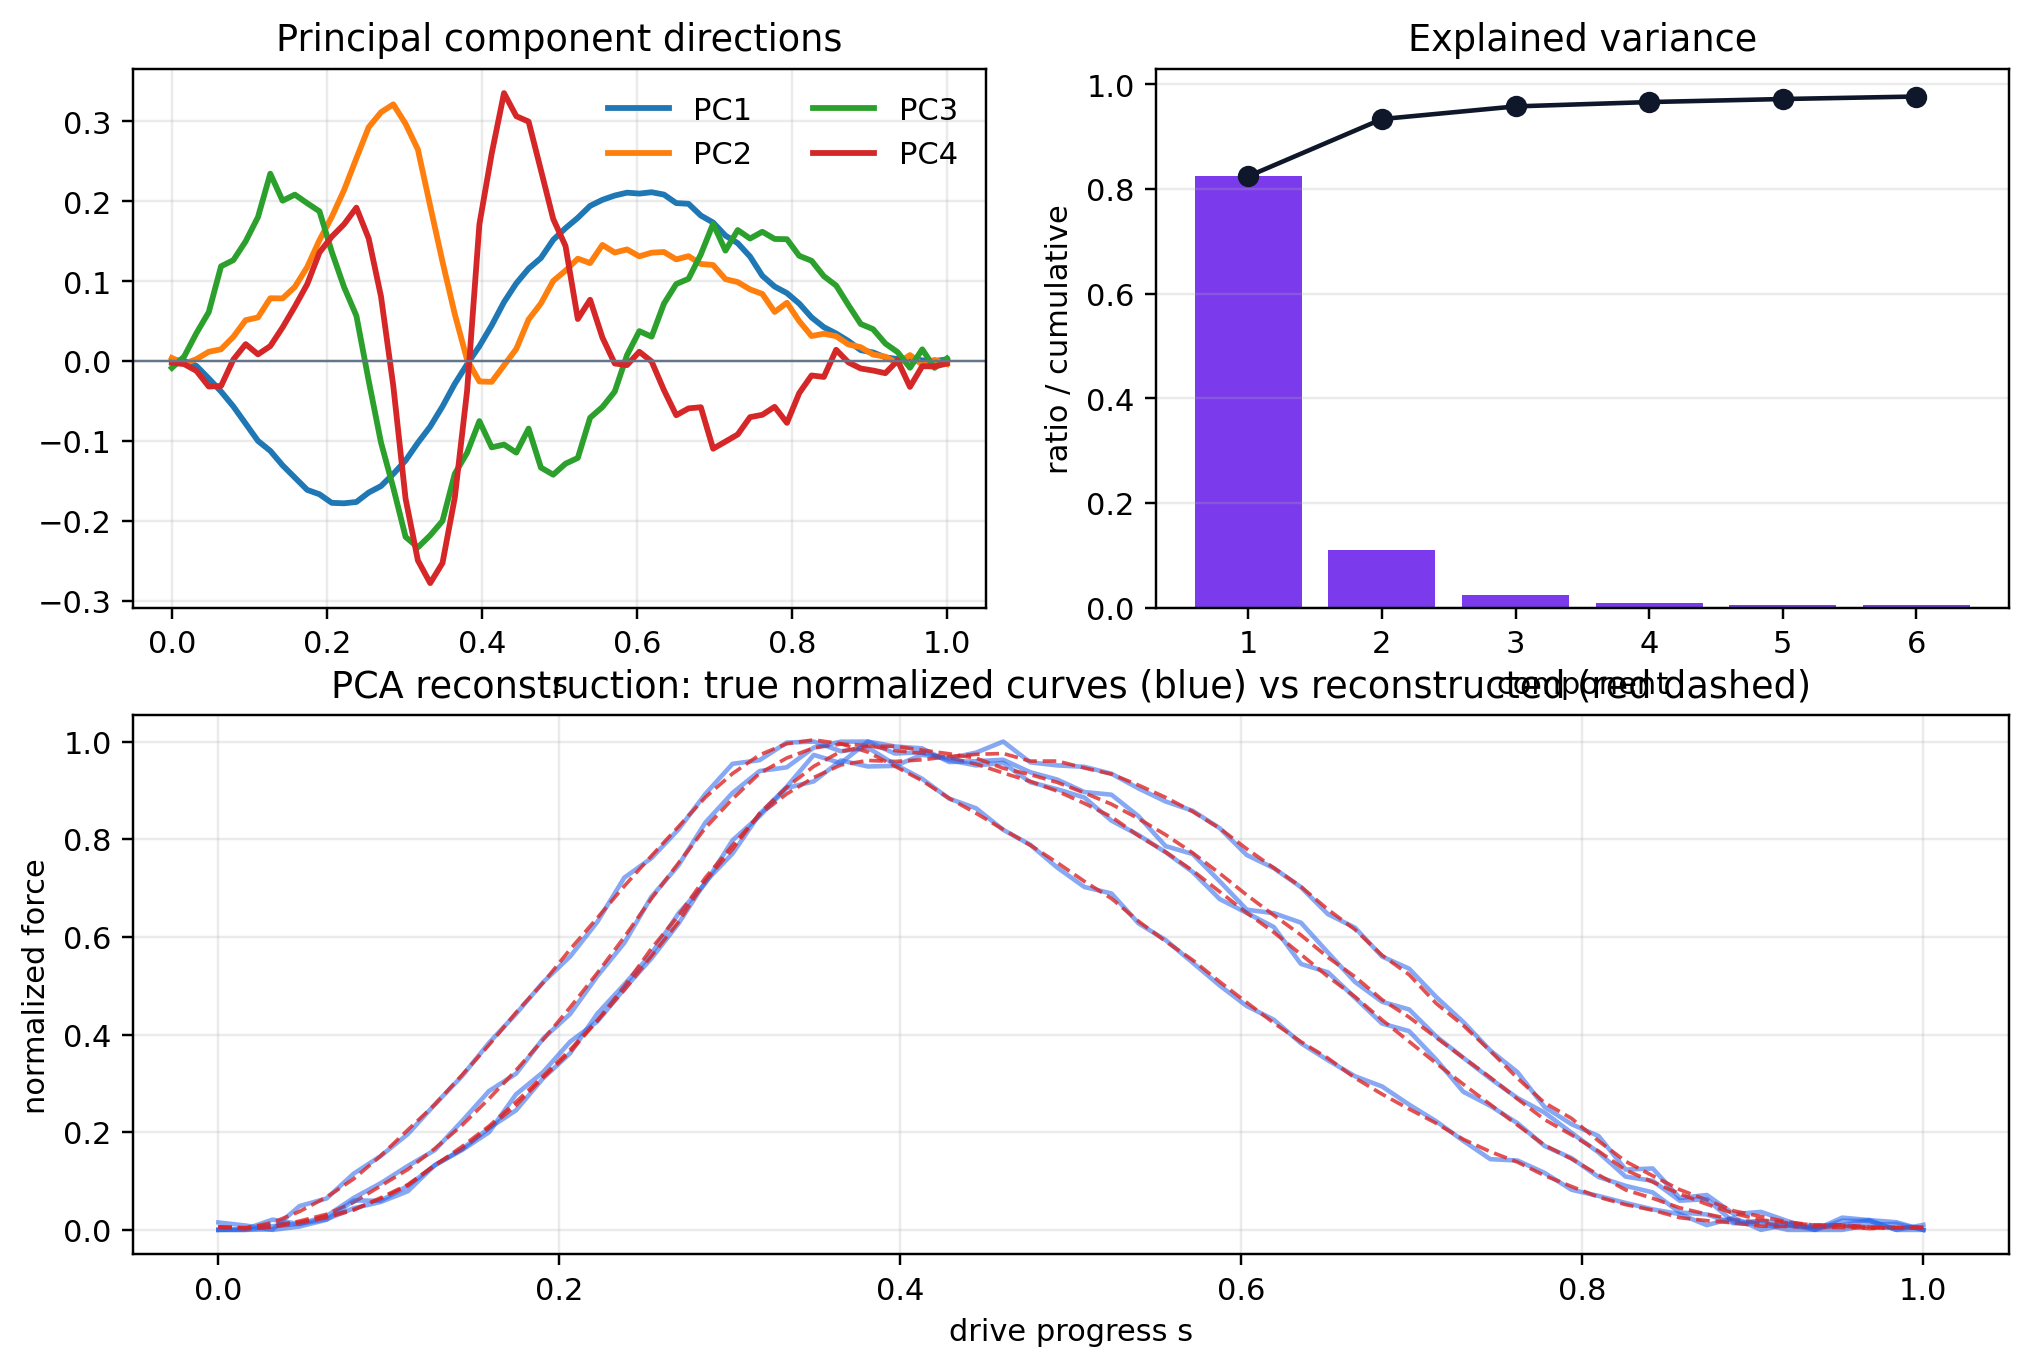
\includegraphics[width=0.96\linewidth]{figures/pca_components.png}
  \caption{PCA components, explained variance, and example reconstructions.}
  \label{fig:pca-components}
\end{figure}

\subsection{Functional PCA}

Standard PCA treats a discretized curve as a vector of \(G\) numbers.
Functional PCA first projects the curve onto a smooth basis, then runs PCA on
the basis coefficients. The implementation in \code{functional_pca.py} uses
cubic B-splines. In simplified notation:
\[
  y_i(s)
  \approx
  \sum_{\ell=1}^{B} a_{i\ell}\phi_\ell(s),
\]
then PCA is applied to the coefficient vectors
\((a_{i1},\ldots,a_{iB})\). This can reduce high-frequency noise before
decomposition.

\clearpage
\section{Evaluation Theory}

\subsection{Why Evaluation Is the Hardest Part}

Training error is easy to reduce. A flexible enough model can memorize small
datasets. The goal is not to minimize error on strokes the model has already
seen; the goal is to estimate how well the learned rule works on new strokes.

For a loss function \(L\), the ideal generalization error is:
\[
  \mathbb{E}_{(X,Y)\sim P_{\text{future}}}
  \left[L(\hat{f}(X),Y)\right].
\]
The distribution \(P_{\text{future}}\) is unknown. Cross-validation approximates
this expectation by repeatedly holding out data, training on the rest, and
measuring held-out error.

\subsection{Cross-Validation Splitters}

The repository implements three split strategies.

\textbf{Time-block split} orders strokes by run and sequence index, then holds
out contiguous blocks. This is useful when data are limited, but train and test
sets may contain the same athlete and even nearby conditions.

\textbf{Session-held-out split} leaves one run out per fold. This is stronger
than random or time-block splitting because the test fold is an entire session.

\textbf{Athlete-held-out split} leaves one athlete out per fold. This is the
strongest split for generalization claims because the test athlete is unseen
during training.

\begin{figure}[H]
  \centering
  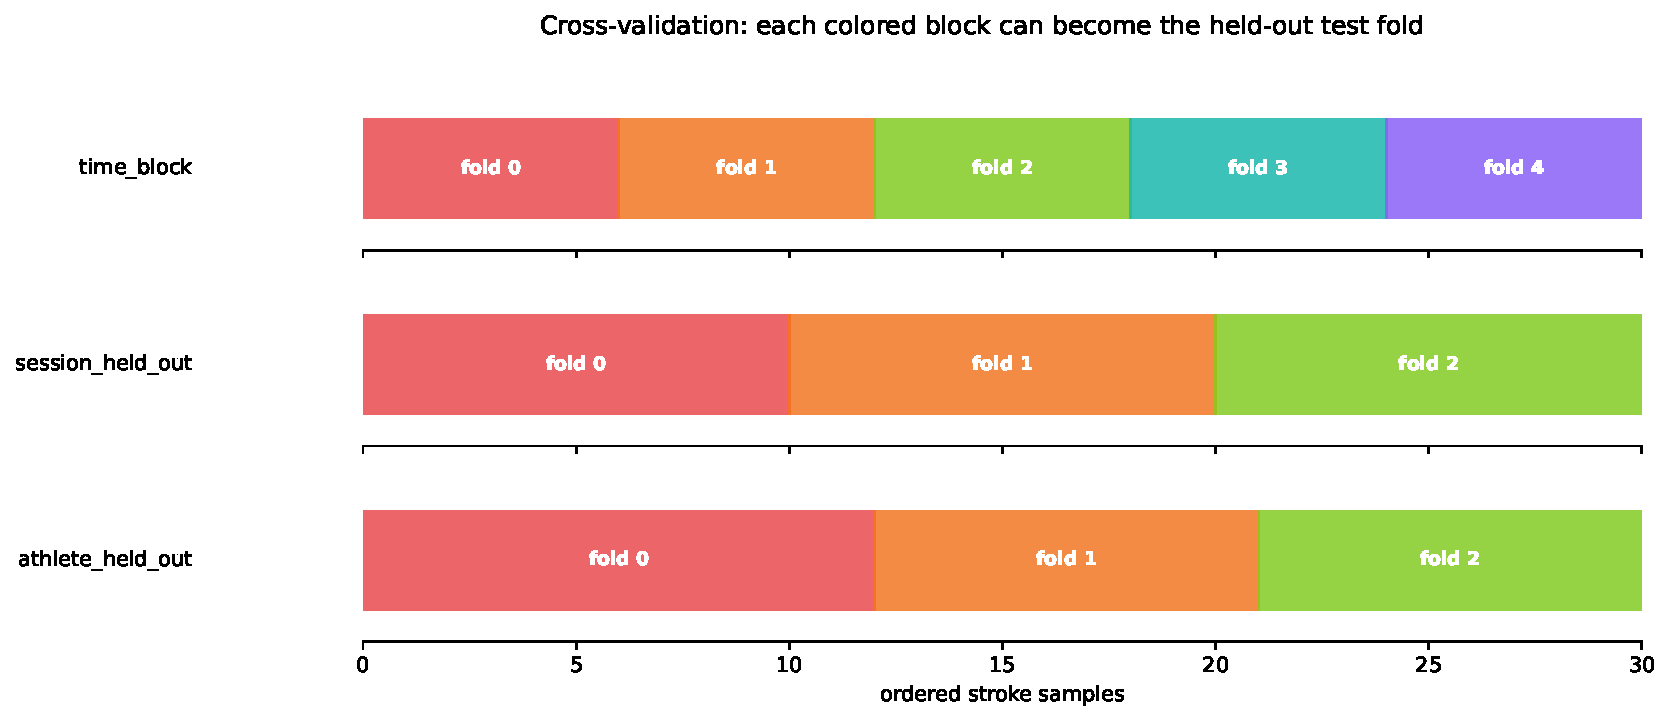
\includegraphics[width=0.95\linewidth]{figures/cv_splits.pdf}
  \caption{Cross-validation split strategies differ in what kind of
  generalization they test.}
  \label{fig:cv-splits}
\end{figure}

\subsection{What Happens Inside One Fold}

A cross-validation fold has two index arrays:
\[
  I_{\text{train}}, \qquad I_{\text{test}}.
\]
The model is fit only with rows in \(I_{\text{train}}\). It then predicts rows
in \(I_{\text{test}}\). Those predictions are written into the global
\code{y_pred_all} array at the held-out indices:

\begin{lstlisting}
for fold_i, (train_idx, test_idx) in enumerate(cv_splitter):
    X_train, X_test = X[train_idx], X[test_idx]
    Y_train, Y_test = Y_pca[train_idx], Y_pca[test_idx]
    model.fit(X_train_s, Y_train_f)
    curves_pred = reconstruct_from_pca(pca_model, model.predict(X_test_s))
    y_pred_all[test_idx] = curves_pred
\end{lstlisting}

This structure matters. A row's final CV prediction is produced by a model that
did not train on that row. At the end, metrics are computed from
\code{force_curves[has_pred]} and \code{y_pred_all[has_pred]}. This is much more
honest than fitting once on the full dataset and reporting in-sample error.

\begin{warningbox}{Leakage}
Leakage occurs when information from the test set influences training. In this
pipeline, leakage can happen if near-duplicate strokes, the same session, or
the same athlete appear in both train and test while the result is interpreted
as broader generalization. The evaluation report labels such results as
provisional.
\end{warningbox}

\subsection{Curve-Level Metrics}

For one stroke with true curve \(y_g\) and predicted curve \(\hat{y}_g\), the
root mean squared error is:
\[
  \operatorname{RMSE}
  =
  \sqrt{\frac{1}{G}\sum_{g=1}^{G} (y_g-\hat{y}_g)^2}.
\]
RMSE penalizes large errors strongly because errors are squared.

The mean absolute error is:
\[
  \operatorname{MAE}
  =
  \frac{1}{G}\sum_{g=1}^{G}|y_g-\hat{y}_g|.
\]
MAE is easier to interpret as an average absolute force error.

Pearson correlation measures shape agreement:
\[
  r =
  \frac{\sum_g (y_g-\bar{y})(\hat{y}_g-\bar{\hat{y}})}
  {\sqrt{\sum_g(y_g-\bar{y})^2}
   \sqrt{\sum_g(\hat{y}_g-\bar{\hat{y}})^2}}.
\]
A model can have high correlation but wrong scale, so correlation is not enough
by itself.

\subsection{Rowing-Relevant Metrics}

The pipeline also computes:
\begin{itemize}[leftmargin=*]
  \item peak force error:
  \[
    \left|\max_g y_g - \max_g \hat{y}_g\right|;
  \]
  \item peak position error:
  \[
    \left|s_{\arg\max y} - s_{\arg\max \hat{y}}\right|;
  \]
  \item impulse error, using trapezoidal integration:
  \[
    \left|\int_0^1 y(s)\,ds - \int_0^1 \hat{y}(s)\,ds\right|;
  \]
  \item early, mid, and late drive MAE.
\end{itemize}

\begin{figure}[H]
  \centering
  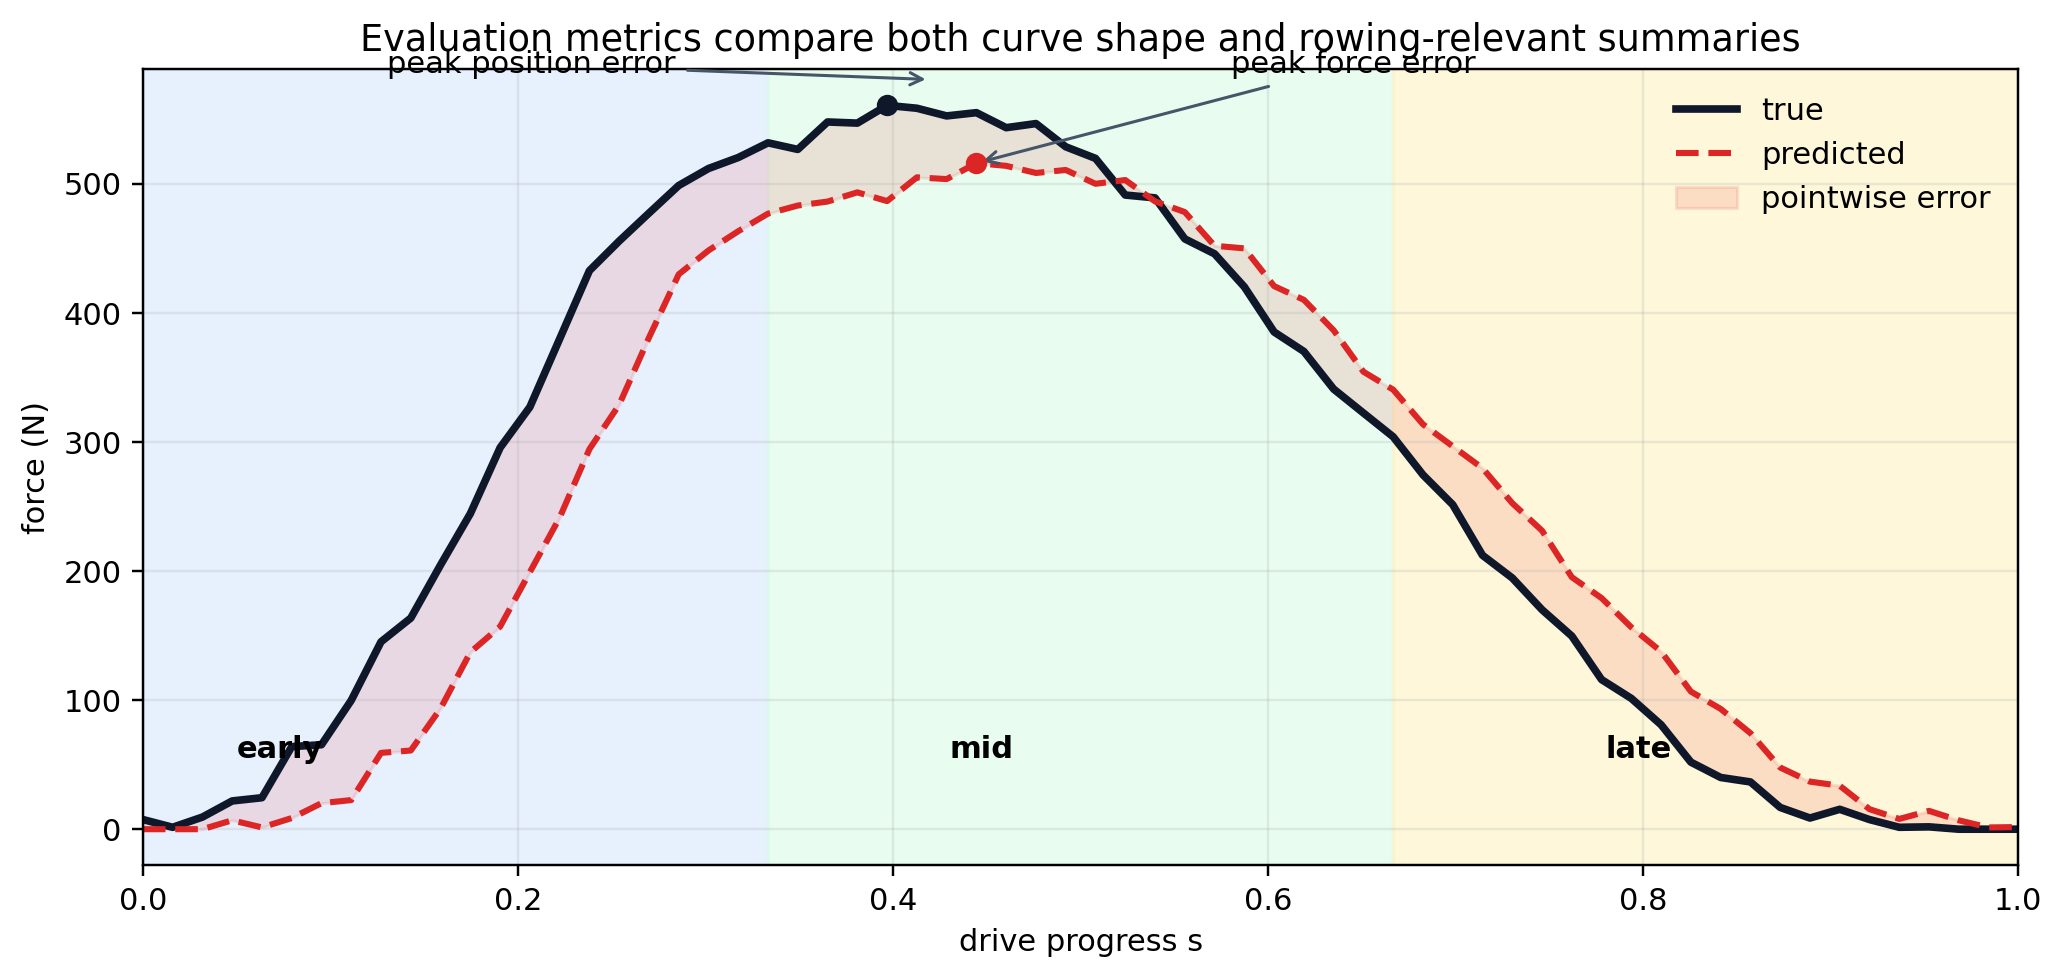
\includegraphics[width=0.95\linewidth]{figures/metrics_diagram.png}
  \caption{Metrics compare both pointwise curve error and rowing-specific
  quantities such as peak force, peak position, and impulse.}
  \label{fig:metrics}
\end{figure}

\subsection{Aggregation}

Metrics are first computed per stroke. The report then aggregates them using
median, mean, and standard deviation. The median is especially useful because a
few badly aligned strokes can dominate the mean.

The code pattern is:
\begin{lstlisting}
metrics = {
    "rmse": rmse_per_stroke(y_true, y_pred),
    "mae": mae_per_stroke(y_true, y_pred),
    "correlation": curve_correlation(y_true, y_pred),
    "peak_force_err": peak_force_error(y_true, y_pred),
}
\end{lstlisting}

\clearpage
\section{Stage 0: Sanity Baselines}

\subsection{Why Stage 0 Exists}

Before claiming that biomechanics predicts force, the pipeline asks two
baseline questions.

First, how reproducible are force curves under similar conditions? If two
strokes with similar rate and length naturally differ by a large amount, then
no model should be expected to beat that noise floor by much.

Second, how much can be predicted from metadata alone? If stroke rate and
stroke length already predict most of the curve, then adding kinematic features
must be judged against that baseline.

\subsection{Force Reproducibility Floor}

The reproducibility function bins strokes by run, stroke rate, and stroke
length. Inside each bin it computes pairwise RMSE between force curves:
\[
  d_{ij}
  =
  \sqrt{\frac{1}{G}\sum_{g=1}^{G}
  \left(Y_i(s_g)-Y_j(s_g)\right)^2}.
\]
It also computes coefficient of variation for peak force and impulse:
\[
  \operatorname{CV}
  =
  \frac{\text{standard deviation}}{\text{mean}}.
\]

\begin{lstlisting}
for i, j in combinations(range(curves_valid.shape[0]), 2):
    d = float(np.sqrt(np.mean((curves_valid[i] - curves_valid[j]) ** 2)))
    pairwise.append(d)
\end{lstlisting}

\subsection{Metadata-Only Ridge Regression}

The metadata baseline predicts PCA coefficients from scalar metadata:
\[
  \vect{x}_i =
  \begin{bmatrix}
  \text{stroke rate}\\
  \text{stroke length}\\
  \text{drive time}
  \end{bmatrix}.
\]
The target is the vector of PCA scores:
\[
  \vect{c}_i =
  \begin{bmatrix}
  c_{i1} & \cdots & c_{iq}
  \end{bmatrix}.
\]

Ridge regression solves:
\[
  \hat{B}
  =
  \arg\min_B
  \sum_i \|\vect{c}_i - \vect{x}_iB\|_2^2
  +
  \alpha\|B\|_F^2.
\]
The penalty discourages very large coefficients, which reduces overfitting
when predictors are correlated or data are limited.

\subsection{Standardization}

Before fitting Ridge, features are standardized:
\[
  z_{ij} = \frac{x_{ij}-\mu_j}{\sigma_j}.
\]
This prevents a large-scale feature such as stroke length in centimeters from
dominating a smaller-scale feature such as drive time in seconds merely because
of units.

\begin{lstlisting}
scaler = StandardScaler().fit(X_train_f)
X_train_s = scaler.transform(X_train_f)
model = Ridge(alpha=1.0)
model.fit(X_train_s, Y_train_f)
\end{lstlisting}

The fitted Ridge model predicts PCA coefficients. Those coefficients are not
the final output shown in the report. The pipeline reconstructs a force curve
and evaluates that curve:
\[
  \vect{x}_i
  \xrightarrow{\text{Ridge}}
  \hat{\vect{c}}_i
  \xrightarrow{\text{PCA inverse}}
  \hat{\vect{Y}}_i.
\]
This is why the same metrics can compare Stage 0, Stage A, and Stage B even
though Stage 0/A predict coefficients and Stage B predicts direct curves.

\subsection{Interpreting a Metadata Baseline}

A strong metadata baseline is not bad news. It means stroke rate, stroke
length, and drive duration contain meaningful information about force shape.
The scientific question becomes sharper: do video-derived biomechanics add
information beyond those simple scalar descriptors?

A weak metadata baseline can also be informative. It may mean the target is
harder than expected, the labels are noisy, or force production varies in ways
not captured by rate and length. In either case, Stage 0 gives context before
adding kinematic complexity.

\subsection{Baseline Gate}

The code defines a baseline gate. A candidate biomechanics model passes only if
it improves curve RMSE and at least one rowing-relevant metric:
\[
  \operatorname{RMSE}_{\text{candidate}}
  <
  \operatorname{RMSE}_{\text{metadata}},
\]
and either peak force error or impulse error improves.

This gate is not a theorem. It is an engineering rule that prevents the project
from mistaking a more complex model for a better model when it fails to beat a
simple baseline.

\clearpage
\section{Stage A: Interpretable Kinematic Baselines}

\subsection{What Stage A Uses}

Stage A uses stroke-level scalar features. It compresses each kinematic curve
into summary statistics:
\[
  \min_s \theta(s),\quad
  \max_s \theta(s),\quad
  \max_s \theta(s)-\min_s \theta(s),\quad
  \frac{1}{G}\sum_g \theta(s_g),\quad
  s_{\arg\max \theta}.
\]
These features are computed for each major angle channel. The resulting table
is easy to inspect, easy to model with classical ML, and easy to interpret.

\subsection{Coordination Features}

The dataset builder also computes coordination features. For a derivative curve
\(d\theta/ds\), onset is defined as the first progress point where the absolute
derivative exceeds a fraction of its peak:
\[
  s_{\text{onset}}
  =
  \min\left\{
  s_g:
  \left|\frac{d\theta}{ds}(s_g)\right|
  \ge
  \rho\max_h
  \left|\frac{d\theta}{ds}(s_h)\right|
  \right\}.
\]
The default threshold fraction is \(\rho=0.15\). Lags such as
\code{lag_knee_to_trunk_s} and \code{lag_trunk_to_arms_s} summarize sequencing
within the drive.

\begin{lstlisting}
threshold = onset_frac * peak
indices = np.where(finite & (abs_d >= threshold))[0]
return float(s_grid[indices[0]])
\end{lstlisting}

\subsection{Stage A Models}

The Stage A code trains three model families:
\begin{itemize}[leftmargin=*]
  \item Ridge regression: stable linear baseline with \(L_2\) penalty.
  \item Lasso regression: linear model with \(L_1\) penalty that can shrink
  some coefficients to zero.
  \item Gradient boosting regressor inside \code{MultiOutputRegressor}: a
  nonlinear tree ensemble trained separately for each PCA target dimension.
\end{itemize}

The input is:
\[
  \vect{x}_i =
  [\text{metadata}, \text{kinematic summaries}, \text{coordination scalars}].
\]
The output is again PCA or fPCA coefficients. Curves are reconstructed before
metrics are computed, so Stage 0 and Stage A are compared on the same force
curve metrics.

\begin{lstlisting}
models = {
    "ridge": lambda: Ridge(alpha=1.0),
    "lasso": lambda: Lasso(alpha=0.01, max_iter=5000),
    "gbr": lambda: MultiOutputRegressor(
        GradientBoostingRegressor(n_estimators=100, max_depth=3)
    ),
}
\end{lstlisting}

The \code{MultiOutputRegressor} wrapper is important. A normal
\code{GradientBoostingRegressor} predicts one target column. PCA targets have
multiple columns, so the wrapper fits one boosted-tree model per coefficient.
This is simple and robust, but it means the model does not explicitly learn
correlations among PCA coefficients.

\subsection{Why Keep Linear Models?}

Even if nonlinear models eventually perform better, linear models are valuable
because they are easier to audit. If Ridge already beats metadata using
kinematic summaries, then there is evidence that the signal is not purely a
high-capacity modeling artifact. If only a flexible tree ensemble improves,
the result may still be real, but it deserves more skepticism and stronger
held-out testing.

\subsection{Feature Importance}

For Ridge and Lasso, importance is based on average absolute coefficient size
across output dimensions:
\[
  I_j = \frac{1}{q}\sum_{\ell=1}^{q}|B_{j\ell}|.
\]
For gradient boosting, importance comes from the underlying tree estimators.
Feature importance is useful for hypothesis generation: it can suggest which
kinematic summaries matter. It should not be overinterpreted as causal proof.

\begin{warningbox}{What Stage A Can and Cannot Prove}
Stage A can show whether compact biomechanics summaries improve prediction over
metadata. It cannot prove that a feature causes force production, and it can
miss information contained in the full shape of the kinematic sequence.
\end{warningbox}

\clearpage
\section{Stage B: Sequence Models}

\subsection{Start Here: Why Stage B Exists}

Stage A collapses each feature curve into a few summary numbers. For example,
a knee-angle curve might become minimum knee angle, maximum knee angle, range,
mean, and the progress point where the maximum occurs. That is useful and
interpretable, but it discards the detailed order of events.

Stage B keeps the full progress-indexed sequence:
\[
  X_i \in \R^{G \times K},
  \qquad
  Y_i \in \R^{G}.
\]
With the default grid, \(G=64\). If there are \(K=14\) kinematic channels, one
stroke is not one row of 14 numbers. It is a \(64 \times 14\) matrix: 64
progress positions, with 14 measurements at each position. The target is a
64-point force curve.

\begin{conceptbox}{The Stage B Question}
Stage B asks: ``Given the whole movement pattern through the drive, can a model
predict the whole force curve?'' It is still supervised regression, but the
input is a sequence and the output is a sequence.
\end{conceptbox}

\subsection{What the Data Looks Like to Stage B}

For one stroke, the input matrix can be read as:
\[
  X_i =
  \begin{bmatrix}
  \text{knee}(s_1) & \text{hip}(s_1) & \cdots & \text{handle accel}(s_1)\\
  \text{knee}(s_2) & \text{hip}(s_2) & \cdots & \text{handle accel}(s_2)\\
  \vdots & \vdots & \ddots & \vdots\\
  \text{knee}(s_G) & \text{hip}(s_G) & \cdots & \text{handle accel}(s_G)
  \end{bmatrix}.
\]
The model output is:
\[
  \hat{Y}_i =
  [\hat{F}(s_1),\hat{F}(s_2),\ldots,\hat{F}(s_G)].
\]

This representation preserves information that summary features cannot fully
capture:
\begin{itemize}[leftmargin=*]
  \item whether knee extension starts before, during, or after trunk swing;
  \item how fast each joint changes during early, middle, and late drive;
  \item whether arms begin drawing while leg drive is still active;
  \item whether force rises gradually, sharply, or in multiple phases;
  \item whether a local change in motion at \(s_g\) predicts a local change in
  force near \(s_g\).
\end{itemize}

\begin{figure}[H]
  \centering
  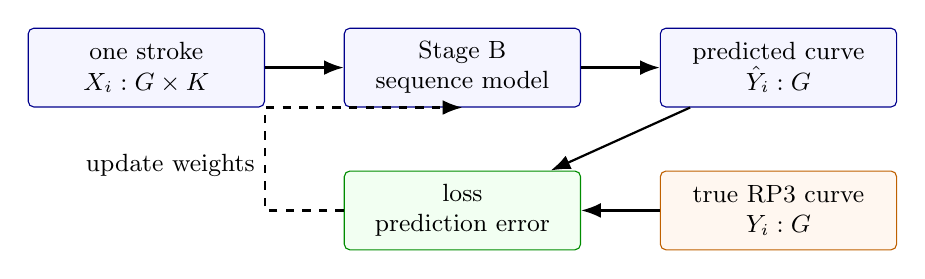
\begin{tikzpicture}[
    font=\small,
    box/.style={draw=blue!55!black, fill=blue!4, rounded corners=2pt,
      minimum height=1.0cm, align=center},
    arrow/.style={-{Latex[length=2.5mm]}, thick}
  ]
    \node[box, minimum width=3.0cm] (x) {one stroke\\\(X_i: G \times K\)};
    \node[box, minimum width=3.0cm, right=1.0cm of x] (model) {Stage B\\sequence model};
    \node[box, minimum width=3.0cm, right=1.0cm of model] (yhat) {predicted curve\\\(\hat{Y}_i: G\)};
    \node[box, minimum width=3.0cm, below=0.8cm of yhat, fill=orange!6,
      draw=orange!75!black] (y) {true RP3 curve\\\(Y_i: G\)};
    \node[box, minimum width=3.0cm, below=0.8cm of model, fill=green!5,
      draw=green!55!black] (loss) {loss\\prediction error};
    \draw[arrow] (x) -- (model);
    \draw[arrow] (model) -- (yhat);
    \draw[arrow] (yhat) -- (loss);
    \draw[arrow] (y) -- (loss);
    \draw[arrow, dashed] (loss.west) -- ++(-1.0,0) |- node[pos=0.22,left]
      {update weights} (model.south);
  \end{tikzpicture}
  \caption{Training compares the predicted force curve with the true RP3 curve.
  The error signal is used to update the model's weights.}
  \label{fig:stageb-learning-loop}
\end{figure}

\subsection{How Stage B Differs From Stage 0 and Stage A}

Stage 0 and Stage A predict PCA or fPCA coefficients. They do not directly
predict every force value. Their flow is:
\[
  \text{features}
  \rightarrow
  \hat{\vect{c}}
  \rightarrow
  \text{PCA inverse transform}
  \rightarrow
  \hat{Y}.
\]

Stage B predicts the force curve directly:
\[
  X_i
  \rightarrow
  \hat{Y}_i.
\]
There is no PCA bottleneck in the Stage B prediction itself. This gives Stage B
more flexibility, because it can represent force-shape details that PCA might
discard. The tradeoff is that Stage B has many more learned parameters, so it
needs stronger controls against overfitting.

\subsection{A Minimal Neural Network Concept}

A neural network is a parametric function. ``Parametric'' means it has numbers
inside it that can be adjusted. Those numbers are called weights and biases.
In the simplest layer:
\[
  \vect{h}
  =
  \sigma(W\vect{x}+\vect{b}),
\]
where \(\vect{x}\) is the input vector, \(W\) is a weight matrix,
\(\vect{b}\) is a bias vector, and \(\sigma\) is a nonlinear activation such as
ReLU:
\[
  \operatorname{ReLU}(u)=\max(0,u).
\]

Without nonlinear activations, stacking many layers would still be only a
linear model. Nonlinearity is what lets a network approximate curved
relationships such as ``force rises when knee extension and trunk swing happen
together, but only during a specific part of the drive.''

\begin{figure}[H]
  \centering
  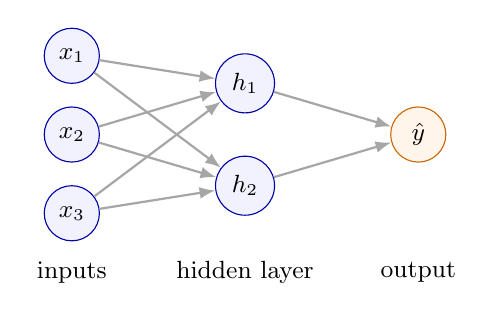
\begin{tikzpicture}[
    font=\small,
    neuron/.style={circle, draw=blue!65!black, fill=blue!5, minimum size=7mm},
    outputnode/.style={circle, draw=orange!80!black, fill=orange!8, minimum size=7mm},
    arrow/.style={-{Latex[length=2mm]}, thick, draw=gray!70}
  ]
    \foreach \i/\y in {1/1.0,2/0.0,3/-1.0} {
      \node[neuron] (x\i) at (0,\y) {\(x_\i\)};
    }
    \foreach \i/\y in {1/0.65,2/-0.65} {
      \node[neuron] (h\i) at (2.2,\y) {\(h_\i\)};
    }
    \node[outputnode] (o) at (4.4,0) {\(\hat{y}\)};
    \foreach \i in {1,2,3} {
      \foreach \j in {1,2} {
        \draw[arrow] (x\i) -- (h\j);
      }
    }
    \foreach \j in {1,2} {
      \draw[arrow] (h\j) -- (o);
    }
    \node[align=center] at (0,-1.75) {inputs};
    \node[align=center] at (2.2,-1.75) {hidden layer};
    \node[align=center] at (4.4,-1.75) {output};
  \end{tikzpicture}
  \caption{A small neural network transforms input numbers through learned
  weighted combinations and nonlinear activations. Stage B applies this idea to
  an entire sequence.}
  \label{fig:small-neural-network}
\end{figure}

\subsection{What ``Learning'' Means}

Learning is not the model gaining understanding in the human sense. Learning
means choosing weights that reduce prediction error on training examples.
At the beginning, the weights are not useful. The model makes predictions,
compares them with the true force curves, computes a loss, and changes the
weights in the direction that reduces that loss.

For a simplified parameter vector \(\vect{\theta}\), the model is
\(\hat{f}_{\vect{\theta}}\). Training solves:
\[
  \hat{\vect{\theta}}
  =
  \arg\min_{\vect{\theta}}
  \frac{1}{N_{\text{train}}}
  \sum_{i \in I_{\text{train}}}
  L\left(\hat{f}_{\vect{\theta}}(X_i),Y_i\right).
\]

The optimizer does this approximately with gradient descent. A gradient tells
the optimizer how the loss changes if each weight changes a little:
\[
  \vect{\theta}_{t+1}
  =
  \vect{\theta}_t
  -
  \eta
  \nabla_{\vect{\theta}} L(\vect{\theta}_t).
\]
Here \(\eta\) is the learning rate. PyTorch computes the gradient with
backpropagation when the code calls \code{loss.backward()}. Backpropagation is
bookkeeping through the chain rule; it tells each weight how much it
contributed to the final error.

\begin{conceptbox}{Plain-English Training Loop}
Predict a force curve, measure how wrong it is, compute which weights caused
the error, nudge those weights, and repeat over many mini-batches.
\end{conceptbox}

\subsection{Mini-Batches and Epochs}

The code does not update the model once per stroke or once for the whole
dataset. It uses mini-batches. If \code{batch_size=32}, each update uses up to
32 strokes at a time:
\[
  X_{\text{batch}} \in \R^{B \times G \times K},
  \qquad
  Y_{\text{batch}} \in \R^{B \times G}.
\]
One epoch means the optimizer has had a chance to see every training stroke
once, split across mini-batches. Stage B may run up to \code{max_epochs}, but
early stopping often ends training sooner.

\subsection{Cross-Validation Still Controls the Claim}

Stage B is trained inside the same cross-validation idea described earlier.
For each fold:
\[
  I_{\text{train}} \cap I_{\text{test}} = \emptyset.
\]
The model may only fit weights using \(I_{\text{train}}\). It predicts
\(I_{\text{test}}\) after training. The final reported CV predictions are
therefore held-out predictions, not in-sample predictions.

Inside the training fold, Stage B also creates a validation split. The code
reserves the last 15 percent of the finite training rows:
\[
  I_{\text{train}}
  =
  I_{\text{fit}} \cup I_{\text{val}}.
\]
\(I_{\text{fit}}\) updates the weights. \(I_{\text{val}}\) decides when to stop
training and which epoch's weights are best. \(I_{\text{test}}\) remains held
out for evaluation.

\begin{figure}[H]
  \centering
  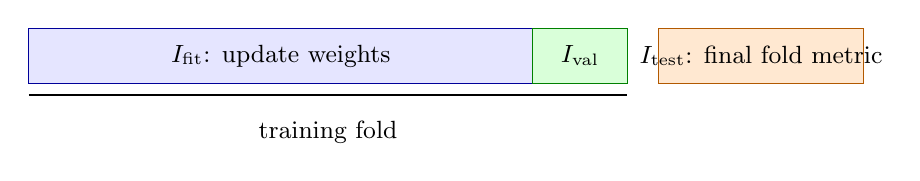
\begin{tikzpicture}[font=\small]
    \draw[fill=blue!10, draw=blue!60!black] (0,0) rectangle (6.4,0.7);
    \draw[fill=green!15, draw=green!50!black] (6.4,0) rectangle (7.6,0.7);
    \draw[fill=orange!18, draw=orange!70!black] (8.0,0) rectangle (10.6,0.7);
    \node at (3.2,0.35) {\(I_{\text{fit}}\): update weights};
    \node at (7.0,0.35) {\(I_{\text{val}}\)};
    \node at (9.3,0.35) {\(I_{\text{test}}\): final fold metric};
    \draw[thick] (0,-0.15) -- node[below=0.2cm]
      {training fold} (7.6,-0.15);
  \end{tikzpicture}
  \caption{The validation rows are inside the training fold. The test fold is
  still held out for the reported cross-validation metrics.}
  \label{fig:stageb-fit-val-test}
\end{figure}

\subsection{What Normalization Does to the Data}

Raw channels have incompatible units and scales. Knee angle is measured in
degrees. Handle acceleration is measured in pixels per second squared. Stroke
coordination channels are fractions of drive progress. If these are fed into a
neural network unchanged, large-unit channels can dominate early training even
when they are not more informative.

Stage B therefore normalizes features channel by channel using only the
training subset:
\[
  z_{igk}
  =
  \frac{x_{igk}-\mu_k}{\sigma_k},
\]
where \(\mu_k\) and \(\sigma_k\) are computed from all finite training values
for channel \(k\). After normalization, each channel is roughly centered near
zero and measured in standard-deviation units.

The target force curve is also normalized:
\[
  y'_{ig}
  =
  \frac{y_{ig}-\mu_y}{\sigma_y}.
\]
The model learns to predict \(y'\), not Newtons directly. After prediction,
the output is converted back to Newtons:
\[
  \hat{y}_{ig}
  =
  \hat{y}'_{ig}\sigma_y+\mu_y.
\]

\begin{figure}[H]
  \centering
  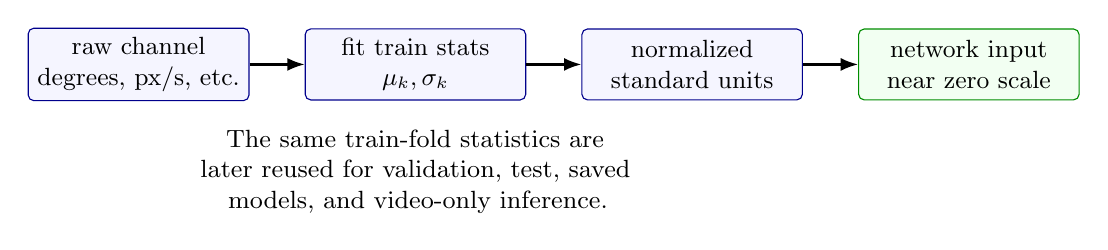
\begin{tikzpicture}[
    font=\small,
    box/.style={draw=blue!55!black, fill=blue!4, rounded corners=2pt,
      minimum height=0.9cm, align=center, minimum width=2.8cm},
    arrow/.style={-{Latex[length=2.2mm]}, thick}
  ]
    \node[box] (raw) {raw channel\\degrees, px/s, etc.};
    \node[box, right=0.7cm of raw] (stats) {fit train stats\\\(\mu_k,\sigma_k\)};
    \node[box, right=0.7cm of stats] (norm) {normalized\\standard units};
    \node[box, right=0.7cm of norm, fill=green!5, draw=green!55!black] (net)
      {network input\\near zero scale};
    \draw[arrow] (raw) -- (stats);
    \draw[arrow] (stats) -- (norm);
    \draw[arrow] (norm) -- (net);
    \node[below=0.25cm of stats, align=center, text width=7.0cm]
      {The same train-fold statistics are later reused for validation, test,
      saved models, and video-only inference.};
  \end{tikzpicture}
  \caption{Normalization changes units, not meaning. A value of \(z=1\) means
  one training-standard-deviation above that channel's training mean.}
  \label{fig:stageb-normalization}
\end{figure}

\begin{warningbox}{Fit Normalization on Training Data Only}
If \(\mu_k\), \(\sigma_k\), \(\mu_y\), or \(\sigma_y\) are computed using test
rows, information leaks from the held-out fold into training. The code avoids
this by fitting normalization after the train/test split inside each fold.
\end{warningbox}

\subsection{Finite-Row Filtering and NaN Handling}

Before Stage B trains a fold, it keeps only training strokes whose full feature
tensor and force curve are finite:

\begin{lstlisting}
finite_train = (
    np.all(np.isfinite(X_train.reshape(X_train.shape[0], -1)), axis=1)
    & np.all(np.isfinite(y_train), axis=1)
)
X_train = X_train[finite_train]
y_train = y_train[finite_train]
\end{lstlisting}

This is a strict filter: a training stroke is removed if any channel at any
grid point is non-finite. The reason is practical. A neural network cannot
multiply by NaN and produce meaningful gradients. A single NaN can contaminate
the loss for the whole mini-batch.

After normalization, arrays sent to the neural network are passed through
\code{np.nan_to_num(..., nan=0.0)}. This mostly protects validation and test
prediction, where some entries can remain missing. Because normalized zero is
the training mean, this replacement means: ``use a typical value for this
missing measurement.'' That is better than crashing, but it is not real
information. Many missing values should still be treated as a data-quality
problem.

\subsection{Optional Coordination Channels}

Stage B can append scalar coordination features to the sequence tensor. A
scalar such as \code{lag_knee_to_trunk_s} has one value per stroke, not one
value per grid point. The code broadcasts it across progress:
\[
  c_i
  \rightarrow
  [c_i,c_i,\ldots,c_i] \in \R^G.
\]
If there are \(C\) coordination scalars, the input shape changes from
\[
  N \times G \times K
  \quad\text{to}\quad
  N \times G \times (K+C).
\]

Broadcasting does not create new time-varying information. It gives the
sequence model stroke-level context at every progress point. For example, the
model can learn different force-shape rules for strokes where arm draw starts
early versus late.

\subsection{The Stage B Shape Contract}

\begin{longtable}{p{0.28\linewidth}p{0.20\linewidth}p{0.42\linewidth}}
\toprule
\textbf{Object} & \textbf{Shape} & \textbf{Meaning}\\
\midrule
\endhead
\code{kinematic_sequences} & \(N \times G \times K\) & Full input tensor before
optional coordination channels.\\
\code{force_curves} & \(N \times G\) & True force targets in Newtons.\\
\code{mask_array} & \(N \times G\) & Boolean valid-target mask; all true when
no mask is supplied.\\
\code{X_train_t} & \(B_{\text{train}} \times G \times K'\) & Normalized PyTorch
training input, where \(K'=K+C\) if coordination channels are used.\\
\code{y_train_t} & \(B_{\text{train}} \times G\) & Normalized force target.\\
\code{model(xb)} & \(B \times G\) & Predicted normalized force curve for a
mini-batch.\\
\code{test_pred} & \(B_{\text{test}} \times G\) & Denormalized held-out
prediction in Newtons.\\
\bottomrule
\end{longtable}

\subsection{Temporal Convolutional Network}

The default Stage B architecture is a temporal convolutional network, or TCN.
``Temporal'' here means sequence-like. The sequence axis is not clock time; it
is normalized drive progress \(s\). A one-dimensional convolution slides a
small window along progress and applies the same learned pattern detector at
each location.

For a single channel, a simple convolution is:
\[
  h_g
  =
  w_{-1}x_{g-1}+w_0x_g+w_{+1}x_{g+1}+b.
\]
With multiple channels, the convolution combines nearby progress points across
all channels. In rowing terms, it can learn local motifs such as:
\[
  \text{``knee angle increasing quickly while trunk angle begins changing.''}
\]

The code's TCN receives data as \(B \times G \times K\), then transposes it for
PyTorch's \code{Conv1d} convention:
\[
  B \times G \times K
  \rightarrow
  B \times K \times G.
\]
The output is transposed conceptually back to a force value at each progress
point.

\begin{figure}[H]
  \centering
  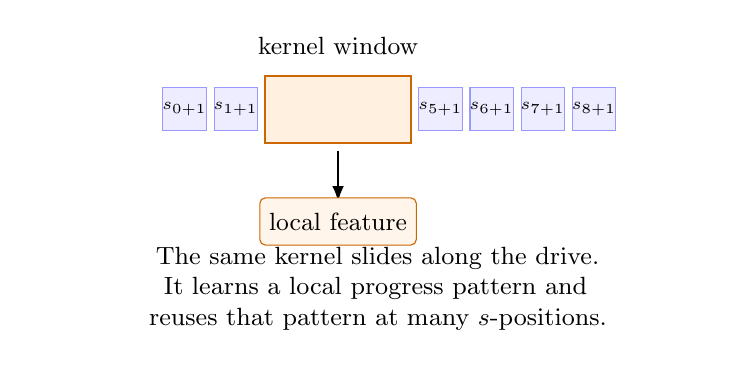
\begin{tikzpicture}[font=\small]
    \foreach \i in {0,...,8} {
      \draw[fill=blue!7, draw=blue!40] (\i*0.65,0) rectangle ++(0.55,0.55);
      \node at (\i*0.65+0.275,0.275) {\(\scriptstyle s_{\i+1}\)};
    }
    \draw[thick, draw=orange!80!black, fill=orange!12] (2*0.65,-0.15)
      rectangle ++(1.85,0.85);
    \node[above=0.15cm] at (2*0.65+0.925,0.7) {kernel window};
    \draw[-{Latex[length=2mm]}, thick] (2*0.65+0.925,-0.25) -- ++(0,-0.65);
    \node[draw=orange!80!black, fill=orange!8, rounded corners=2pt,
      minimum width=1.6cm, minimum height=0.6cm] at (2*0.65+0.925,-1.15)
      {local feature};
    \node[align=center, text width=8.6cm] at (2.7,-2.0)
      {The same kernel slides along the drive. It learns a local progress
      pattern and reuses that pattern at many \(s\)-positions.};
  \end{tikzpicture}
  \caption{A 1D convolution looks at a local neighborhood along the drive
  progress axis.}
  \label{fig:stageb-convolution-window}
\end{figure}

\subsection{Dilations and Receptive Field}

If a convolution only sees immediate neighbors, it may miss wider coordination
patterns. A dilated convolution skips positions:
\[
  h_g
  =
  \sum_r W_r x_{g+rd}.
\]
When the dilation \(d=1\), the kernel sees adjacent positions. When \(d=2\), it
samples every second position. When \(d=4\), it samples every fourth position.
The Stage B TCN stacks blocks with dilations:
\[
  1,\;2,\;4,\;8,\ldots
\]
so deeper layers can combine information from a larger portion of the stroke.

This is important for rowing because force at mid-drive may depend on how the
early drive unfolded. The model needs some way to connect local force
prediction with earlier or later body-motion context.

\subsection{Residual Connections, BatchNorm, and Dropout}

The TCN block contains several practical neural-network tools.

\textbf{Residual connections} add a block's input back to its output. In
simplified form:
\[
  \text{output} = \operatorname{Block}(x) + x.
\]
This helps optimization because a block can learn a correction to an existing
representation rather than having to rebuild the whole representation from
scratch.

\textbf{Batch normalization} rescales intermediate activations during training.
It makes the distribution of hidden values more stable, which often makes
training faster and less sensitive to initialization.

\textbf{Dropout} randomly zeros some hidden activations during training. This
prevents the network from relying too heavily on one fragile pathway through
the model. At inference time, dropout is disabled.

\subsection{Transformer Encoder}

The Transformer is the alternative Stage B architecture. It uses self-attention
instead of sliding convolution windows. The first step projects each
progress-point feature vector into a hidden embedding:
\[
  \vect{e}_g = W_{\text{in}}\vect{x}_g+\vect{b}_{\text{in}}.
\]
The model then adds a positional encoding, because otherwise the same feature
vector at catch and finish would look too similar to the Transformer:
\[
  \vect{e}'_g = \vect{e}_g + \vect{p}_g.
\]

Self-attention lets each progress point compare itself with every other
progress point. In matrix form:
\[
  \operatorname{Attention}(Q,K,V)
  =
  \operatorname{softmax}
  \left(\frac{QK^\top}{\sqrt{d}}\right)V.
\]
For study purposes, read this as:
\begin{itemize}[leftmargin=*]
  \item \(Q\), queries: what each progress point is looking for;
  \item \(K\), keys: what each progress point offers for comparison;
  \item \(V\), values: the information copied and mixed after attention scores
  are computed.
\end{itemize}

\begin{figure}[H]
  \centering
  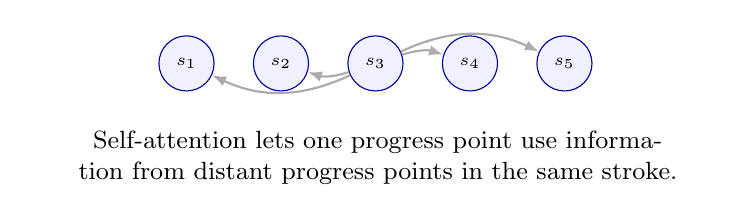
\begin{tikzpicture}[
    font=\small,
    point/.style={circle, draw=blue!60!black, fill=blue!6, minimum size=7mm},
    arrow/.style={-{Latex[length=1.8mm]}, draw=gray!65, thick}
  ]
    \foreach \i/\x in {1/0,2/1.2,3/2.4,4/3.6,5/4.8} {
      \node[point] (s\i) at (\x,0) {\(\scriptstyle s_\i\)};
    }
    \draw[arrow] (s3) to[bend left=25] (s1);
    \draw[arrow] (s3) to[bend left=18] (s2);
    \draw[arrow] (s3) to[bend left=18] (s4);
    \draw[arrow] (s3) to[bend left=25] (s5);
    \node[align=center, text width=8.6cm] at (2.4,-1.2)
      {Self-attention lets one progress point use information from distant
      progress points in the same stroke.};
  \end{tikzpicture}
  \caption{A Transformer can connect early, middle, and late drive positions
  directly.}
  \label{fig:stageb-attention}
\end{figure}

The Transformer can capture long-range coordination patterns. It also has more
ways to overfit when the dataset is small. In this project, it should be judged
against the TCN and the simpler Stage 0/A baselines with held-out metrics, not
by architectural sophistication.

\subsection{Masked MSE and Derivative Loss}

Stage B's core loss is pointwise mean squared error. If all target force values
are valid, it is:
\[
  L_{\text{MSE}}
  =
  \frac{1}{NG}
  \sum_{i,g}(\hat{y}_{ig}-y_{ig})^2.
\]
When a mask is supplied, invalid target positions are ignored:
\[
  L_{\text{MSE}}
  =
  \frac{\sum_{i,g}m_{ig}(\hat{y}_{ig}-y_{ig})^2}
  {\sum_{i,g}m_{ig}}.
\]
Here \(m_{ig}=1\) means the target is valid and \(m_{ig}=0\) means it should
not contribute to the loss.

An optional derivative penalty compares first differences:
\[
  L_{\Delta}
  =
  \frac{1}{N(G-1)}
  \sum_{i,g}
  \left[
  (\hat{y}_{i,g+1}-\hat{y}_{ig})
  -
  (y_{i,g+1}-y_{ig})
  \right]^2.
\]
This does not merely ask ``is the force value right?'' It also asks ``is the
local change in force right?'' That can discourage predictions with the right
average level but the wrong rise and fall shape.

The full loss is:
\[
  L = L_{\text{MSE}} + \lambda L_{\Delta}.
\]
If \(\lambda=0\), the derivative term is disabled. If \(\lambda\) is too high,
the model may over-prioritize curve slope at the expense of force magnitude.

\subsection{What AdamW, Weight Decay, and Scheduling Do}

The code trains with AdamW:
\begin{lstlisting}
optimizer = torch.optim.AdamW(model.parameters(), lr=lr,
                              weight_decay=weight_decay)
\end{lstlisting}
AdamW is a gradient-based optimizer. Compared with plain gradient descent, it
keeps adaptive running scales for parameters, so weights with noisy or small
gradients can still be updated effectively.

Weight decay discourages large weights. It is a regularizer:
\[
  \text{large weights} \quad \Rightarrow \quad \text{slightly higher objective}.
\]
This can reduce overfitting because extremely large weights often indicate that
the model is fitting narrow details of the training set.

The cosine scheduler changes the learning rate over epochs:
\begin{lstlisting}
scheduler = torch.optim.lr_scheduler.CosineAnnealingLR(
    optimizer, T_max=max_epochs
)
\end{lstlisting}
Early training can use larger steps. Later training uses smaller steps, which
helps the optimizer settle rather than bounce around.

\subsection{Gradient Clipping}

Neural-network gradients can occasionally become very large. A huge gradient
can cause one update to damage the model. The code clips gradient norm:
\begin{lstlisting}
loss.backward()
torch.nn.utils.clip_grad_norm_(model.parameters(), 1.0)
optimizer.step()
\end{lstlisting}
This keeps an update from becoming too large even if one mini-batch produces an
unstable gradient.

\subsection{Training Loop in Code Terms}

For each cross-validation fold, Stage B:
\begin{enumerate}[leftmargin=*]
  \item selects train and test strokes;
  \item optionally appends coordination scalars as broadcast sequence channels;
  \item filters training rows with finite features and targets;
  \item reserves the last 15 percent of the finite training fold as validation
  data;
  \item computes feature and target normalization from the fit subset;
  \item normalizes train, validation, and test inputs with the same statistics;
  \item replaces remaining normalized NaNs with zero;
  \item builds either the TCN or Transformer;
  \item trains with mini-batches, masked MSE, optional derivative loss, AdamW,
  cosine scheduling, and gradient clipping;
  \item monitors validation loss and restores the best epoch;
  \item predicts the held-out test fold;
  \item denormalizes predictions back to Newtons;
  \item stores those predictions in \code{y_pred_all[test_idx]}.
\end{enumerate}

The important scientific detail is the final one. Each row in
\code{y_pred_all} is filled by a model that did not train on that row.

\begin{figure}[H]
  \centering
  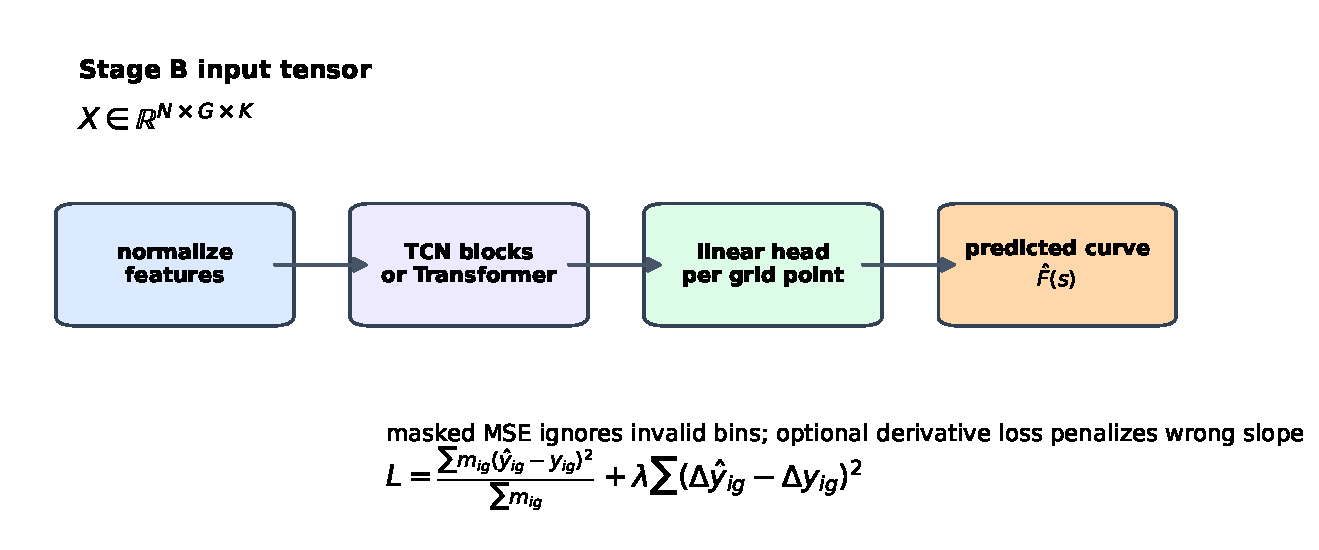
\includegraphics[width=0.95\linewidth]{figures/stageb_architecture.pdf}
  \caption{Stage B maps the full progress-aligned feature tensor to a full
  force curve.}
  \label{fig:stageb}
\end{figure}

\subsection{Early Stopping}

Early stopping is a practical guard against overfitting. During training,
validation loss is monitored. If it does not improve for \code{patience}
epochs, training stops and the best validation state is restored.

This matters because neural networks can keep improving on the training set
while getting worse on held-out data:
\[
  L_{\text{train}} \downarrow
  \qquad
  \text{but}
  \qquad
  L_{\text{val}} \uparrow.
\]
That pattern means the network is learning details that do not generalize.
The validation subset is not the final test fold; it is a tuning signal inside
the training fold.

\subsection{Overfitting: The Main Risk in Stage B}

Stage B is powerful because it can learn from the whole \(G \times K\) tensor.
That same power is the risk. If there are few athletes or few sessions, a
large sequence model may memorize camera angle, athlete-specific rhythm,
session-specific rig setup, or label noise.

Signs of overfitting include:
\begin{itemize}[leftmargin=*]
  \item training loss improves but validation loss worsens;
  \item time-block CV looks good but athlete-held-out CV looks poor;
  \item predicted curves look too similar to the average curve;
  \item predicted curves have plausible RMSE but wrong peak timing or impulse;
  \item Stage B does not beat Stage 0/A despite being much more flexible.
\end{itemize}

The correct response is not automatically to make Stage B larger. Often the
right response is better alignment, stricter QC, more sessions, stronger
held-out splits, or simpler architecture.

\subsection{What Gets Saved}

The best Stage B fold state is saved as a PyTorch state dictionary, not as a
complete Python object:
\begin{itemize}[leftmargin=*]
  \item \code{stageB_tcn_state.pt} or \code{stageB_transformer_state.pt}: learned
  weights.
  \item \code{stageB_tcn_arch.json} or \code{stageB_transformer_arch.json}:
  architecture parameters needed to rebuild the model class.
  \item \code{stageB_tcn_norm.npz} or \code{stageB_transformer_norm.npz}:
  feature and target normalization constants.
\end{itemize}
For downstream compatibility, the code also writes the canonical
\code{stageB_tcn_*} filenames even when the selected architecture is the
Transformer. The architecture JSON records what kind of model should actually
be rebuilt.

This design is more portable than pickling a whole neural network object. The
model bundle later combines these files with the feature contract and PCA
artifacts so video-only prediction can reproduce the training-time transforms.

\subsection{Inference After Training}

During video-only inference, the trained Stage B model no longer has RP3 force
curves. The inference path must reproduce the same feature construction and
normalization:
\[
  \text{video}
  \rightarrow
  X_{\text{new}}
  \rightarrow
  \frac{X_{\text{new}}-\mu_X}{\sigma_X}
  \rightarrow
  \hat{Y}'
  \rightarrow
  \hat{Y}'\sigma_y+\mu_y.
\]
The saved normalization constants are therefore part of the model. A neural
network's weights are not enough; the input coordinate system must match the
one used during training.

\subsection{How to Read Stage B Results}

When Stage B results are written, read them in this order:
\begin{enumerate}[leftmargin=*]
  \item Check the evaluation regime: time-block, session-held-out, or
  athlete-held-out.
  \item Check whether Stage B beats the metadata-only Stage 0 baseline.
  \item Check whether it beats Stage A, not only whether it trains.
  \item Inspect RMSE and MAE for pointwise force error.
  \item Inspect peak force error, peak position error, and impulse error for
  rowing relevance.
  \item Inspect true-vs-predicted curves to see whether the model predicts
  realistic curve shapes.
\end{enumerate}

\begin{conceptbox}{The Practical Interpretation}
A useful Stage B model is not simply one with low training loss. It is one that
turns video-derived movement sequences into held-out force curves that improve
on simple metadata and summary-feature baselines under the strongest split the
dataset can support.
\end{conceptbox}

\clearpage
\section{Reading Results}

\subsection{Output Files}

The training script writes JSON, NumPy, and model artifacts under the modeling
output directory.

\begin{longtable}{p{0.34\linewidth}p{0.56\linewidth}}
\toprule
\textbf{File} & \textbf{Use}\\
\midrule
\endhead
\code{stage0_reproducibility.json} & Within-condition force variability and
noise-floor statistics.\\
\code{stage0_metadata_baseline.json} & Metadata-only metrics and fold
statistics.\\
\code{stageA_results.json} & Stage A metrics, feature columns, feature
importance, and baseline gate status.\\
\code{stageB_results.json} & Stage B architecture, fold metrics, and overall
metrics.\\
\code{cv_predictions/*.npy} & Held-out predictions assembled across CV folds.\\
\code{comparison_summary.json} & Model comparison rows from the current run.\\
\code{evaluation_report.json} & Unified evaluation regime, alignment integrity,
and model results.\\
\code{evaluation_report.txt} & Human-readable version of the evaluation report.\\
\bottomrule
\end{longtable}

\subsection{How to Decide Whether a Model Improved}

Use this checklist:
\begin{enumerate}[leftmargin=*]
  \item Did the model beat the metadata-only Stage 0 baseline on median RMSE?
  \item Did it improve at least one rowing-relevant metric such as peak force
  error or impulse error?
  \item Was the split appropriate for the claim? Time-block is not the same as
  athlete-held-out.
  \item Are alignment metrics acceptable? Bad labels can make model metrics
  meaningless.
  \item Are results consistent across folds, or driven by one lucky fold?
  \item Does the model produce plausible curves, not just good aggregate
  numbers?
\end{enumerate}

\subsection{Reports}

The report generator reads the modeling artifacts and creates an HTML training
report. The report includes stage metrics, residual plots, true-vs-predicted
overlays, cohort summaries, leakage warnings, and provenance. Treat it as the
dashboard, but remember that the source of truth is still the saved artifacts.

\clearpage
\section{Code-Based Labs}

The companion notebooks live in \code{study_guide/notebooks}. Each notebook
checks for an environment variable:
\[
  \code{DATASET_DIR=/path/to/training_dataset}.
\]
If that directory exists, the notebook loads real artifacts. Otherwise it
generates synthetic data with the same shapes and column names.

\begin{labbox}{Lab Map}
\begin{itemize}[leftmargin=*]
  \item \code{01_dataset_contract.ipynb}: inspect tables, tensors, and shapes.
  \item \code{02_progress_features.ipynb}: visualize progress interpolation and
  derivatives.
  \item \code{03_pca_force_curves.ipynb}: fit PCA and reconstruct curves.
  \item \code{04_cv_and_metrics.ipynb}: compute metrics and compare split
  logic.
  \item \code{05_stage0_stageA.ipynb}: train small Ridge, Lasso, and gradient
  boosting baselines.
  \item \code{06_stageB_toy_model.ipynb}: demonstrate masked loss and a tiny
  sequence model when PyTorch is available.
\end{itemize}
\end{labbox}

\subsection{Suggested Study Workflow}

For each lab, use the same routine:
\begin{enumerate}[leftmargin=*]
  \item Run the notebook once with synthetic data so it is guaranteed to
  execute.
  \item Set \code{DATASET_DIR} to a real training dataset and rerun.
  \item Compare the real shapes and plots against the synthetic version.
  \item Find the corresponding code block in the repository.
  \item Write down one question about why that implementation choice was made.
\end{enumerate}

The purpose of the notebooks is not to replace the repo. They are controlled
experiments that isolate one concept at a time: shape contracts, interpolation,
PCA, metrics, baselines, and sequence loss.

\section{Code Reading Checklist}

When reading a new function in this repository, use the following sequence:
\begin{enumerate}[leftmargin=*]
  \item Identify the input type: DataFrame, NumPy array, model object, or file
  path.
  \item Write down the expected shape of every major array.
  \item Identify which rows are filtered and why.
  \item Check whether normalization is fit on training data only.
  \item Check whether the function mutates data, writes artifacts, or just
  returns objects.
  \item Ask whether the operation belongs to feature construction, target
  construction, model fitting, or evaluation.
\end{enumerate}

This checklist is deliberately mechanical. Complex pipelines become easier to
understand when every function is reduced to inputs, outputs, shape changes,
and statistical role.

\appendix

\section{Formula Reference}

\subsection{Ridge Regression}
\[
  \hat{B}
  =
  \arg\min_B
  \|Y-XB\|_F^2+\alpha\|B\|_F^2.
\]
Ridge is useful when predictors are correlated and sample size is limited.

\subsection{Lasso Regression}
\[
  \hat{B}
  =
  \arg\min_B
  \|Y-XB\|_F^2+\alpha\|B\|_1.
\]
Lasso can shrink coefficients to zero, creating a sparse linear model.

\subsection{PCA Reconstruction}
\[
  \hat{\vect{y}}
  =
  \vect{\mu}
  +
  \sum_{j=1}^{q} \hat{c}_j \vect{v}_j.
\]
Stage A predicts \(\hat{c}_j\), then reconstructs \(\hat{\vect{y}}\).

\subsection{Trapezoidal Impulse}
\[
  \operatorname{Impulse}
  \approx
  \sum_{g=1}^{G-1}
  \frac{y_g+y_{g+1}}{2}(s_{g+1}-s_g).
\]
The code uses \code{np.trapz}.

\section{Package Glossary}

\begin{description}[leftmargin=0.28\linewidth, style=nextline]
  \item[\code{numpy}] Dense numerical arrays, vectorized math, interpolation,
  gradients, and saving/loading \code{.npy} files.
  \item[\code{pandas}] Tables, CSV loading, grouping by stroke, metadata
  columns, and scalar feature tables.
  \item[\code{scikit-learn}] PCA, StandardScaler, Ridge, Lasso, Gradient
  Boosting, and multi-output wrappers.
  \item[\code{PyTorch}] Stage B neural sequence models, training loops,
  autograd, optimizers, and saved state dictionaries.
  \item[\code{joblib}] Serialization for scikit-learn models such as PCA and
  fitted regressors.
  \item[\code{matplotlib}] Diagnostic plots and report figures.
\end{description}

\section{Common Failure Modes}

\subsection{Bad Alignment}
If video strokes are matched to the wrong RP3 rows, the model learns from wrong
labels. Always check cumulative catch error, interval error, and stroke-rate
agreement before trusting model metrics.

\subsection{Too Little Data}
With few athletes or sessions, flexible models can memorize. Prefer simpler
baselines until held-out evaluation is stable.

\subsection{Noisy Derivatives}
Derivatives amplify pose jitter. If derivative channels dominate feature
importance or cause poor Stage B behavior, inspect smoothing and QC flags.

\subsection{Average-Curve Collapse}
A model can reduce MSE by predicting a generic average curve. True-vs-predicted
overlays and peak/impulse metrics help catch this.

\subsection{Misleading Split}
A good time-block score does not imply cross-athlete generalization. The
evaluation regime label should match the claim being made.

\section{Minimal Reading Path}

If you are short on time, read in this order:
\begin{enumerate}[leftmargin=*]
  \item Sections 1 and 2 for the supervised-learning contract.
  \item Section 3.5 through 3.8 for force targets and PCA.
  \item Section 4 for evaluation and leakage.
  \item Section 5 for the baseline gate.
  \item Section 7 for Stage B training mechanics.
  \item Section 8 for reading results.
\end{enumerate}

\end{document}
